\documentclass[prd,aps,letter,twocolumn,floatfix,notitlepage,nofootinbib]{revtex4-1}

%% packages
\usepackage{graphicx,psfrag}
\usepackage{mathrsfs,amsmath,amsfonts,amssymb, bm}
\usepackage{multirow}
\usepackage{comment,hyperref}
\usepackage{float}
\usepackage{algorithm}
\usepackage{algpseudocode} % in place of algorithmic. Conflicts with revtex4 unless [H] option passed
\usepackage{setspace} % for pleasent spacing in algorithm
\usepackage{times}
\usepackage{ulem}

%% macros
\newcommand{\be}{\begin{equation}}
\newcommand{\ee}{\end{equation}}
\newcommand{\bsube}{\begin{subequations}}
\newcommand{\esube}{\end{subequations}}

%\def\l{\ell}
%\def\blambda{{\bm \lambda}}
%\def\bLambda{{\bm \Lambda}}
%\def\blam{\bar{\lambda}}
%\def\Lam{\Lambda}
%\def\Lamt{\tilde{\Lambda}}
%\def\dLamt{\tilde{\delta{\Lambda}}}
%\def\bmu{{\bm \mu}}

\def\bx{\mathbf{x}}
\def\btheta{\boldsymbol{\theta}}



%% macros for comments
\usepackage{color}
%% colors
\definecolor{cyan}{rgb}{0,0.9,0.9}
\definecolor{orange}{rgb}{0.9,0.5,0}
\definecolor{magenta}{rgb}{1,0,1}
\definecolor{purple}{rgb}{0.8,0.4,0.8}
\definecolor{gray}{rgb}{0.8242,0.8242,0.8242}
%%
\newcommand{\bs}[1]{{\textcolor{green}{\texttt{SB: #1}} }}
\newcommand{\bl}[1]{{\textcolor{blue}{\texttt{BL: #1}} }}
\newcommand{\cg}[1]{{\textcolor{orange}{{CG: #1}} }}
\newcommand{\cvdb}[1]{{\textcolor{purple}{\texttt{CVDB: #1}} }}
\newcommand{\red}[1]{\textcolor{red}{#1}}
\newcommand{\blue}[1]{\textcolor{blue}{#1}}
%% +++++++++++++++++++++++++++++++++++++++++++++++++++++++
\begin{document}

\title{Surrogate model of aligned-spin binary neutron star waveforms using Gaussian process regression}

\author{
Benjamin D. Lackey$^1$, 
Michael P\"{u}rrer$^1$
Andrea Taracchini$^1$
}
\affiliation{
$^1$Max Planck Institute for Gravitational Physics, Albert Einstein Institute, D-14476 Golm, Germany
} 

\date{\today}

\begin{abstract}

Fast and accurate waveform models are necessary for measuring properties of inspiraling binary neutron star systems such as the masses, spins, and tidal parameters. The effective one body (EOB) formalism has been used to produce BNS waveforms that include aligned-spin, quadrupolar and octopolar adiabatic tides, as well as the effect of dynamical tides, and the formalism is accurate enough to avoid significant biases in the measured parameters. Unfortunately, current implementations take several minutes to a day to evaluate, and this is too slow for parameter estimation codes that require $10^7$--$10^8$ sequential waveform evaluations. We construct a frequency-domain surrogate of this model that requires less than 0.3~s to evaluate for a waveform with a starting frequency of 10~Hz (0.04~s for a starting frequency of 30~Hz). We first reduce the 12-dimensional intrinsic parameter space of this model to the 5-dimensional parameter space that includes mass ratio, aligned-spins, and quadrupolar tides using universal relations that approximate all matter effects in terms of the leading quadrupolar tidal parameter. We then use Gaussian process regression and active learning to optimally sample the parameter space and construct a surrogate with $\sim 1000$ waveforms instead of the $\gtrsim 10^5$ waveforms that would be required with standard, grid-based interpolation methods. 

For the parameter most sensitive to waveform errors, the tidal parameter, we find that the error from the resulting surrogate leads to a systematic error in the measured tidal parameter $\tilde\Lambda$ of less than $\sim 50$ which is less than 10\% of typical tidal parameters.


\end{abstract}

\pacs{
  % 04.25.D-,   % numerical relativity
  % 
  04.30.Db,   % gravitational wave generation and sources
  % 04.40.Dg,   % Relativistic stars: structure, stability, and oscillations
  % 04.70.Bw,   % classical black holes
  95.30.Sf,     % relativity and gravitation
  % 
  % 95.30.Lz,   % Hydrodynamics
  % 97.60.Jd    % Neutron stars
  % 97.60.Lf    % black holes (astrophysics)
  % 98.62.Mw    % Infall, accretion, and accretion disks
}

%%
\maketitle


%% ________________________________________________________
\section{Introduction}

\red{[[What is possible with BNS systems:]]}

The detection of the binary neutron star (BNS) system GW170817 [[cite]] by the Advanced LIGO [[cite]] and Advanced Virgo [[cite]] gravitational-wave detectors, has demonstrated that the sky position, distance, masses, spins, and tidal parameters can be measured with enough precision to answer fundamental physics questions such as identifying BNS mergers as a source of gamma ray bursts [[cite]], measuring the Hubble constant [[cite]], and understanding the structure of neutron stars (NSs) through tidal interactions [[cite]]. Measuring these parameters accurately will also be necessary to properly interpret the gamma ray burst [[cite]] and optical afterglow [[cite]] that was found in conjunction. Furthermore, an estimate of the BNS merger rate of x--y events Gpc$^{-3}$~yr$^{-1}$ (90\% confidence interval) [[GW170817]] indicates that, when second generation detectors reach design sensitivity, including KAGRA [[cite]] and possibly LIGO-India [[cite]], we could eventually observe a population of tens or hundreds of events after a couple of years of observation [[2010Rates?]]. This will allow us to estimate the NS mass distribution [[cite]], spin distribution [[cite]], and universal equation of state (EOS) that is common to all NSs [[DelPozzo, Lackey, ...]]. 

\red{[[Why we need more accurate waveform models to do these things:]]}

These results are obtained using a Bayesian analysis that compares the data to parameterized waveform templates. To avoid systematic errors highly accurate waveform templates are needed. In addition, the Bayesian parameter estimation alogrithms (Markov chain Monte Carlo and Nested Sampling [[parallel algorithms are becoming available]]) typically perform several million sequential waveform evaluations, requiring waveform evaluation times to be less than $\mathcal{O}(1s)$ in order to run in less than a month for each event.

%The primary quantities of interest for BNS merger observations are the sky position, masses, spins, and tidal parameters. These parameters, measured with Bayesian parameter estimation techniques, require highly accurate waveform models to avoid systematic errors. For example, post-Newtonian (PN) waveform models, which are truncated at the currently known 3.5PN order, lead to uncertainties in the waveform phase of approximately 10~rad up to a merger frequency of $\sim 1000$~Hz [[cite]]. This is approximately the same size as the contribution to the phase from tidal effects, and as a result, the systematic errors in the measured tidal parameter are as large as the tidal parameter itself [[cite]]. This also biases the recovered NS equation of state and radius [[cite]], as well as the masses and spins [[cite]].


\red{[[The problems with the current waveform models/templates.]]}

To date, there are a limited number BNS waveform models that include spin and tides, and that are fast enough for standard parameter estimation.  
TaylorF2: (not so good point particle. okay tidal terms)
For example, post-Newtonian (PN) waveform models, which are truncated at the currently known 3.5PN order, lead to uncertainties in the waveform phase of approximately 10~rad up to a merger frequency of $\sim 1000$~Hz [[cite]]. This is approximately the same size as the contribution to the phase from tidal effects, and as a result, the systematic errors in the measured tidal parameter are as large as the tidal parameter itself [[cite]]. This also biases the recovered NS equation of state and radius [[cite]], as well as the masses and spins [[cite]].

\*\_NRTides: (better/good point particle. better tidal terms)
Initial parameter estimation results for the first BNS event, GW170817 using a variety of waveform templates (TaylorF2, SEOBNRv4\_ROM\_NRTides, and IMRPhenomD\_NRTides) showed that there are noticeable differences in the measured parameters between the different waveform templates [[cite]], and in particular the tidal parameter. [[NR\_Tides is a fit to NR waveforms at high frequency and has only been fit to a limited number of low spin, low tidal parameter NR simulations.]]

TEOBResumS:

\red{[[What is good about the new EOB model:]]}

The effective one body (EOB) formalism, on the other hand, has significantly smaller uncertainties than PN waveforms. Variations within the EOB formalism lead to uncertainties in the waveform phase of $\sim 1$~rad [[cite or say as shown below]] as compared to PN waveform uncertainties of $\sim 10$~rad. Furthermore, NR simulations of BNS systems now claim phase errors of less than 1~rad during the last $\sim 10$ orbits through merger [[cite]] and show good agreement with EOB models [[cite]]. 

Another model 


\red{[[Problem with EOB (speed). Attempts to speed it up with optimization. Alternative using surrogates.]]}

Unfortunately, available implementations for generating EOB waveforms for BNS systems take anywhere from 10 minutes to a day to evaluate for a single waveform with a starting GW frequency of 10Hz [[cite]]. Bayesian parameter estimation algorithms such as Markov-chain Monte Carlo and nested sampling, however, typically require $10^7$--$10^8$ sequential waveform evaluations, making current EOB implementations unusable. Significant work has been done to optimize existing implementations of EOB for BBH systems [[EtienneMcWilliams]]. However, it is not clear that these optimizations can be readily adapted for the BNS model discussed here with dynamical tides. We therefore develop a surrogate model that accelerates the evaluation of EOB waveforms by interpolating between a sparsely sampled training set of waveforms within the parameter space. 

Surrogate modeling techniques have had significant success in gravitational-wave data analysis for accelerating the evaluation of a waveform $h(t;\bx)$ given its waveform parameters $\bx$. The standard technique is to construct a training set of waveforms that sample the parameter space, then compress this training set by building a reduced, orthonormal basis whose linear combination can reproduce any waveform in the parameter space to some desired accuracy. This serves to interpolate the waveform as a function of time (or frequency for frequency-domain waveforms) in terms of a reduced set of coefficients corresponding to the reduced set of basis functions. In previous work, this reduced basis has been constructed either with singular value decomposition (SVD) [[Michael's papers]] or with a greedy method that chooses a subset of the training-set waveforms that are as orthogonal to each other as possible, then orthonormalizes this subset with Graham-Schmidt orthogonalization [[All the other papers]].

\red{[[Overview of surrogates. Typical methods that have been used. Their problems. What you are doing that is new.]]}








%The effective one body (EOB) formalism, on the other hand, has significantly smaller uncertainties than PN waveforms. Variations within the EOB formalism lead to uncertainties in the waveform phase of $\sim 1$~rad [[cite or say as shown below]] as compared to PN waveform uncertainties of $\sim 10$~rad. Furthermore, NR simulations of BNS systems now claim phase errors of less than 1~rad during the last $\sim 10$ orbits through merger [[cite]] and show good agreement with EOB models [[cite]]. Unfortunately, available implementations for generating EOB waveforms for BNS systems take anywhere from 10 minutes to a day to evaluate for a single waveform with a starting GW frequency of 10Hz [[cite]]. Bayesian parameter estimation algorithms such as Markov-chain Monte Carlo and nested sampling, however, typically require $10^7$--$10^8$ sequential waveform evaluations, making current EOB implementations unusable. Significant work has been done to optimize existing implementations of EOB for BBH systems [[EtienneMcWilliams]]. However, it is not clear that these optimizations can be readily adapted for the BNS model discussed here with dynamical tides. We therefore develop a surrogate model that accelerates the evaluation of EOB waveforms by interpolating between a sparsely sampled training set of waveforms within the parameter space. 

%Surrogate modeling techniques have had significant success in gravitational-wave data analysis for accelerating the evaluation of a waveform $h(t;\bx)$ given its waveform parameters $\bx$. The standard technique is to construct a training set of waveforms that sample the parameter space, then compress this training set by building a reduced, orthonormal basis whose linear combination can reproduce any waveform in the parameter space to some desired accuracy. This serves to interpolate the waveform as a function of time (or frequency for frequency-domain waveforms) in terms of a reduced set of coefficients corresponding to the reduced set of basis functions. In previous work, this reduced basis has been constructed either with singular value decomposition (SVD) [[Michael's papers]] or with a greedy method that chooses a subset of the training-set waveforms that are as orthogonal to each other as possible, then orthonormalizes this subset with Graham-Schmidt orthogonalization [[All the other papers]].

Once this reduced basis is built, one can interpolate each of the coefficients $c_i(\bx)$ as a function of the waveform parameters $\bx$. This method has been used for frequency-domain surrogates of aligned spin BBH waveforms [[Michael's papers]]. Alternatively, one can use the empirical interpolation method (EIM) [[cite]] which re-expresses the linear combination of orthonormal basis functions in terms of a sum of empirical interpolating functions $B_j(t)$ times the value of the waveform $h(T_j; \bx)$ at empirical nodes $T_j$. One then interpolates the waveform $h(T_j; \bx)$ as a function of $\bx$ at each node $T_j$. This method has been used for time domain-waveforms for nonspinning [[cite]], aligned-spin [[cite]], and precessing [[cite]] BBH waveforms as well as nonspinning BNS waveforms with tidal interactions [[cite]], and frequency-domain, precessing waveforms [[cite]].

Previous work on surrogate models has focused mainly on parameter spaces $\bx$ with $\le 3$~dimensions. This allows one to approximate the coefficients $c_i(\bx)$ or waveform values $h(T_j; \bx)$ as functions of $\bx$ using simple fitting functions [[cite]] or standard interpolation techniques such as tensor spline [[Michael, others]] or Chebyshev interpolation [[Ben]]. These interpolation techniques typically require waveforms evaluated on a rectangular grid, and this suffers from the curse of dimensionality; for $N$ points per dimension $d$,  $N^d$ waveforms are needed. For the 5-dimensional problem here, this is somewhat unfeasable. Recent work on optimally choosing waveforms for both EOB [[cite GPRpaper]] and NR [[cite CaltechPrecessing]] waveforms has shown that there are sufficiently accurate alternatives to grid-based interpolation that do not suffer from the curse of dimensionality.

In this paper we focus on breaking this curse of dimensionality by using an interpolation method known as Gaussian process regression (GPR) that does not require a regular grid. Importantly, GPR also provides a convenient estimate of its own uncertainty. This allows us to iteratively add new points to the training set in such a way as to minimize the interpolation error over the parameter space for a given number of waveforms in the training set. A similar approach has recently been used to optimally sample waveforms for a 2-dimensional parameter space using GPR [[DoctorEtAl]]. GPR has also been used recently in GW data analysis to marginalize over waveform uncertainties in parameter estimation [[ChrisMoore2papers?]].

In this paper, we will develop methods to construct a surrogate model for the inspiral through merger of an aligned spin BNS waveform with tidal interactions using the EOB tidal description described in Hinderer et al.~[[cite1, cite2]]. This work is a continuation of the surrogate developed in [[cite]] for a nonspinning BNS waveform using a slightly different description for the point-particle and tidal pieces by Bernuzzi et al.~[[cite, ...]]. Whereas in [[Ben]] we constructed a time-domain surrogate with the goal of reproducing the original waveform model as accurately as possible, in this work, we construct a frequency-domain model which significantly speeds up parameter estimation by not requiring an online Fourier transform for each waveform evaluation. It also enables additional techniques such as reduced order quadrature [[cite]] to accelerate likelihood evaluation.

\red{[[Obligitory summary:]]}

We organize the paper as follows. In Section II we provide an overview of the EOB waveform model used for constructing the surrogate and the approximations we use to reduce the dimensionality of the parameter space. In section III, we describe the details of building a surrogate model, choosing training set waveforms, and evaluating the final model. We then compare the accuracy and speed of the surrogate to the original model in section IV. Then, finally discuss future improvements and applications in Section V.

\textit{Conventions:} Unless explicitly stated, we use units where $G=c=1$. To agree with the GPR literature, we will refer to the waveform parameters as $\bx$ and the hyperparameters in the GPR model as $\btheta$.

\red{[[In the introduction you should emphasize the parts of this paper that are new to the GW field: Applying GPR to a high dimensional parameter space, showing that you can choose several new training set samples then calculate them in parallel without reconstructing the reduced basis. Building a surrogate for the residual to reduce the required interpolation accuracy. The first BNS waveform that realistically tapers to zero amplitude. Active learning method that readily extends to higher dimensions. By attaching to TaylorF2, the surrogate is valid for all frequencies.]]}

\red{[[We aim to construct a sufficiently accurate waveform surrogate using as few waveform evaluations as possible, to show how one could use NR simulations/go to higher dimensions.]]}

%% ________________________________________________________
\section{Aligned-spin, dynamical tides EOB model}

\red{[[Say somewhere that this model is based off of what is known as SEOBNRv4 (and/or 2?) in lalsuite.]]}

\red{[[The inspiral part is exactly as described in previous papers. The post-merger part is new to this paper. If this is true, we should write that somewhere.]]}

The effective-one-body (EOB) approach to the general-relativistic 2-body problem, first described in Ref.~\cite{Buonanno:1998gg}, has proven successful in modeling the dynamics and GW emission of binaries of compact objects. State-of-the-art aligned-spin EOB models~\cite{Bohe:2016gbl,Nagar:2017jdw} can accurately match hundreds of numerical-relativity (NR) simulations of aligned-spin binary black holes (BBHs) for mass ratios up to 8 and spin magnitudes up to 0.85 for unequal-mass (up to 0.98 for equal-mass) binaries. The EOB framework can also accommodate precessing-spin BBHs, showing good agreement to mildly precessing NR simulations~\cite{Babak:2016tgq}. This research program has been extended to accommodate tidal effects~\cite{Damour:2009wj,Vines:2010ca,Damour:2012yf,Bini:2012gu,Bernuzzi:2014owa,Hinderer:2016eia,Steinhoff:2016rfi,Dietrich:2017feu}, which become especially relevant in the strong-field regime for 2-body systems that contain matter---BNS or neutron-star-black-hole (NSBH) binaries. The main effect of tides is to make the gravitational interaction more attractive with respect to the vacuum case. In particular, Refs.~\cite{Hinderer:2016eia,Steinhoff:2016rfi} built upon the aligned-spin BBH EOB model of Ref.~\cite{Taracchini:2013rva} and proposed a way to include the effect of dynamical tides. Neutron stars that are part of a compact-object binary will deform in the tidal field generated by the companion---be it a black hole or another neutron star. Because of binary motion, the forcing tidal field varies at the orbital frequency. Thus, in the late stages of the inspiral, the characteristic $f$-mode frequency of the neutron star can be dynamically approached, resulting in a resonant excitation of the f-mode. The net effect is an amplification of tidal effects as compared to the adiabatic limit, which assumes that the $f$-mode frequency is much larger than the frequency of the forcing tidal field. 

We note that, to date, this is the only tidal EOB model that includes the effect of spin \red{[[Sebastiano also has a model that includes spin and tides.]]}\blue{[[Which is the Reference?]]}. More precisely, spin effects are those of the point-mass part of the model~\cite{Bohe:2016gbl}, that was calibrated to 141 NR simulations of aligned-spins BBHs.\footnote{This model is implemented in the LIGO Algorithm Library as SEOBNRv4.} The model, however, does not account for the quadrupole that the neutron stars acquire when they are spinning. This is a genuine matter effect that appears at lower PN order as compared to the tidal effects that are currently modeled. The importance of this physical effect in the context of data analysis for ground-based GW interferometers is currently being studied~\cite{IanTanja}.

\subsection{Inspiral-plunge waveform}

Dynamical tidal effects are implemented in the EOB model through a modification of the potential $\Delta_u$, which is the $tt$-component of the metric of the effective spacetime. \red{[[Show how $\Delta_u$ enters the Hamiltonian.]]}\blue{[[There's no easy/illuminating way to explain how this potential enters the Hamiltonian]]}. In this paper we adopt the tidally-augmented expression of $\Delta_u$ that is discussed in Appendix~A of Ref.~\cite{Steinhoff:2016rfi}, namely
\begin{equation}
\Delta_u = \Delta_u^{\textrm{pm}} + \Delta_u^{\textrm{DT}}\,,
\end{equation}
where $\Delta_u^{\textrm{pm}}$ is the 4PN-accurate point-mass term of the underlying BBH EOB model of Ref.~\cite{Bohe:2016gbl} (see Eq.~(2.2) therein) and $\Delta_u^{\textrm{DT}}$ is the contribution due to dynamical tides. We consider the general case of a binary that may consist of two neutron stars; if either component of the binary is a black hole, then vanishing values of the tidal polarizabilities are employed in the formulas below. Let $A$ and $B$ be the body labels. Let $M_{A,B}$ be the mass of either body and $M=M_A+M_B$ be the total mass of the binary.  Explicitly, including quadrupolar and octupolar tidal effects, we have
\begin{widetext}
\begin{align}
 \Delta_u^{\textrm{DT}} =&  - 3\,\Lambda_{2,\textrm{dyn}}^{A}(u)X_A^4 X_B\,u^6  \left[ 1 + \frac{5}{2} X_Au + \left(3 + \frac{1}{8}X_A + \frac{337}{28} X_A^2\right)u^2 \right]\nonumber\\
 &- 15\,\Lambda_{3,\textrm{dyn}}^{A}(u)X_A^6X_B\,u^8 \left[1 + \left(-2 + \frac{15}{2}X_A\right)u + \left(\frac{8}{3} - \frac{311}{24}X_A + \frac{110}{3}X_A^2\right) u^2\right] + (A \leftrightarrow B)\,,
\end{align}
\end{widetext}
where $X_{A,B}=M_{A,B}/M$, $u=1/r$ is the inverse of the ($M$-rescaled) EOB radial coordinate $r$ and $\Lambda_{\ell,\textrm{dyn}}^{A,B}(u)$ are the dimensionless $2^{\ell}$-polar dynamical tidal polarizabilities. Within the dynamical tides model, the tidal polarizabilities are not constant, but rather depend on the orbital separation and on the values of the $f$-mode frequencies $\hat{\omega}_{0\ell}^{A,B}$. In particular, the dimensionless dynamical tidal polarizability reads
\begin{equation}
\Lambda_{\ell,\textrm{dyn}}^{A,B}(u)=\Lambda_{\ell}^{A,B}\hat{k}_{\ell\,\textrm{dyn}}(u;\hat{\omega}_{0\ell}^{A,B})\,,
\end{equation}
where $\Lambda_{\ell}^{A,B}$ is the dimensionless adiabatic tidal polarizability
\begin{equation}
\Lambda_{\ell}^{A,B}=\frac{2}{(2\ell-1)!!}\frac{k^{A,B}_{\ell}}{C_{A,B}^{2\ell+1}}\,,
\end{equation}
with $k^{A,B}_{\ell}$ the tidal Love number and $C_{A,B}=R_{A,B}/M_{A,B}$ the neutron star compactness, which depends on the areal radius $R_{A,B}$ of the neutron star. Here $\hat{k}_{\ell\,\textrm{dyn}}(u;\hat{\omega}_{0\ell}^{A,B})$ is the separation-dependent, dimensionless enhancement factor given in Eq.~(11) of Ref.~\cite{Dietrich:2017feu}, which depends on the value of the $f$-mode $2^\ell$-pole dimensionless angular frequency, $\hat{\omega}_{0\ell}^{A,B}$.\footnote{Here $\hat{\omega}_{0\ell}^{A,B}=M_{A,B}\omega_{0\ell}^{A,B}$, where $\omega_{0\ell}^{A,B}$ is the frequency in geometrized units.} This enhancement factor is 1 for low orbital frequencies, and increases to about 2 as $\ell$ times the orbital frequency approaches the $f$-mode frequency. 

Tidal effects also enter the dissipative part of the model. In particular, the point-mass $\ell=2,3$ inspiral-plunge waveform modes are corrected by tidal terms
\begin{equation}
h_{\ell m}^{\textrm{insp-plunge}} = h_{\ell m}^{\textrm{pm}} + h_{\ell m}^{\textrm{tidal}}\,,\label{hlminspplunge}
\end{equation} 
where the point-mass piece $h_{\ell m}^{\textrm{pm}}$ is discussed in Section~II.B of Ref.~\cite{Bohe:2016gbl} and the tidal piece $h_{\ell m}^{\textrm{tidal}}$ is given by Eqs. (A14)-(A17) of Ref.~\cite{Damour:2012yf}. Following Ref.~\cite{Dietrich:2017feu} in the computation of $h_{22}^{\textrm{tidal}}$, we include a dynamical enhancement factor that depends on the orbital separation and on the $f$-mode frequency, and is given in Eq.~(15) of Ref.~\cite{Dietrich:2017feu}. The waveform modes $h_{\ell m}^{\textrm{insp-plunge}}$ are then used to calculate the GW flux (Eqs.~(5) and (6) in Ref.~\cite{Dietrich:2017feu}) from which the radiation-reaction force is derived.

Let us now discuss the construction of the full waveform. The Hamiltonian equations of motion with the above radiation-reaction force are numerically integrated beginning with the quasicircular initial conditions described in Ref.~\cite{Buonanno:2005xu}. The inspiral-plunge waveform is obtained by evaluating Eq.~(\ref{hlminspplunge}) using the solution to the orbital dynamics. Let $\Omega$ be the instantaneous orbital frequency, $r$ be orbital separation, $p_r$ be the radial momentum, $f_s$ be the waveform sampling frequency in Hz, $\omega_{\textrm{peak}}^{\textrm{NR}}$ be the NR fit for the (2,2)-mode amplitude peak of a BNS merger defined in Eq.~(2) of Ref.~\cite{Bernuzzi:2015rla}~\footnote{Note that this fit was tuned to NR simulations only for $0 \leq \kappa_2^T \leq 500$, where $\kappa_2^T$ is defined by Eq.~(1) of Ref.~\cite{Bernuzzi:2015rla}. In our model, for $\kappa_2^T >500$ we use the value of this fit at $\kappa_2^T=500$.}. Then the numerical integration of the orbital dynamics stops when any of the following events happens: (i) $\Omega$ peaks, (ii) $p_r$ becomes positive, (iii) $\dot{r}$ becomes positive, (iv) $\dot{p}_r$ becomes positive, (v) $r$ does not evolve more than a 1000th of the leading-order estimate for $\dot{r}$, that is $\propto 64/5 \nu/r^4$, (vi) $2\Omega$ reaches $\omega_{\textrm{peak}}^{\textrm{NR}}$, (vii) $2M\Omega$ reaches $\pi M f_s$. In order to avoid triggering these stopping conditions at low frequency, where residual orbital eccentricity due to imperfect quasicircular initial conditions could be present, we exploit the $\omega_{\textrm{peak}}^{\textrm{NR}}$ fit to define a radius below which the stopping conditions can be triggered; such threshold value is taken to be $1.5 (\omega_{\textrm{peak}}^{\textrm{NR}}/2)^{-2/3}$.  

Let $t_{\textrm{peak}}^{\textrm{amp}}$ be the earliest time when the amplitude of the $(\ell,m)=(2,2)$ mode $|h_{22}^{\textrm{insp-plunge}}|$ peaks, and let $t_{\textrm{peak}}^{\textrm{freq}}$ be the time when the inspiral-plunge GW frequency $\omega_{22}^{\textrm{insp-plunge}}$ is maximum. Then
\begin{equation}
t_{\textrm{match}}^{22} = \min \left(t_{\textrm{peak}}^{\textrm{amp}},t_{\textrm{peak}}^{\textrm{freq}}\right)\,.\label{tmatch}
\end{equation}
If $|h_{22}^{\textrm{insp-plunge}}|$  does not peak, then we choose $t_{\textrm{peak}}^{\textrm{amp}}$ to be the earliest time when $\partial_t |h_{22}^{\textrm{insp-plunge}}|$ reaches a minimum after having reached a peak.

In the BBH model, nonquasicircular corrections to the inspiral-plunge signal guarantee that the waveform peaks at a prescribed time and has prescribed amplitude and frequency, hence $t_{\textrm{match}}^{22}=t_{\textrm{peak}}^{\textrm{amp}}$. Here, however, we do not impose such corrections because of limited input from NR BNS simulations, therefore we have little control over the behavior of Eq.~(\ref{hlminspplunge}) in the late inspiral. This motivates our choice of $t_{\textrm{match}}^{22}$ in Eq.~(\ref{tmatch}), with the goal of reducing to the BBH prescription in the non-tidal limit and avoiding non-monotonic growth of the GW frequency in the late inspiral. To help bracket the stopping time, we exploit a fit for the (2,2)-mode peak frequency of NR BNS simulations~\cite{Bernuzzi:2015rla} to estimate the final orbital frequency of the EOB inspiral-plunge dynamics. %When such frequency is being approached (to within some tolerance), we stop the numerical evolution if a peak in the orbital frequency is detected or if the binary stops to monotonically plunge, similarly to what is done in the BBH case. 
In our model we only include the dominant $(\ell,m)=(2,2)$ mode in constructing the final waveform, although we use all modes when evaluating the radiation reaction force.

Ref.~\cite{Dietrich:2017feu} carried out comprehensive comparisons of this model to state-of-the-art NR simulations of coalescing nonspinning BNSs with different mass ratios and equations of state, finding that the model can accurately describe the GW phasing up to the last cycle before merger for systems with soft equation of state, while improvements are still needed for systems with stiff equation of state. Similar results hold for the tidal EOB model of Ref.~\cite{Bernuzzi:2014owa}, whose radial potential includes tidal effects in a form that is inspired by first-order gravitational-self-force (GSF) calculations of tidal invariants in the small-mass-ratio limit. Both the EOB model with dynamical tides and the GSF-inspired one are significantly more faithful to NR than the adiabatic tidal EOB model of Refs.~\cite{Damour:2009wj,Bini:2012gu}.

\subsection{Post-merger waveform}

We model the post-merger GW emission that tapers to zero amplitude in terms of analytic functions for the amplitude $A_{22}^{\textrm{post-mrg}}(t)$ and phase $\phi^{\textrm{post-mrg}}(t)$ such that $h_{22}^{\textrm{post-mrg}}(t) = A_{22}^{\textrm{post-mrg}}(t) \exp{[i\phi_{22}^{\textrm{post-mrg}}(t)]}$. For the amplitude, we define the following linear extension of the inspiral-plunge amplitude
\begin{align}
\hat{A}(t)=\left\{\begin{array}{ll}
|h_{22}^{\textrm{insp-plunge}}(t)|, & t \leq t^{22}_{\textrm{match}}\,, \\
a + b (t-t^{22}_{\textrm{match}}) , & t > t^{22}_{\textrm{match}}\,,
\end{array}\right.
\end{align}
where $a=|h_{22}^{\textrm{insp-plunge}}(t^{22}_{\textrm{match}})|$ and $b=\partial_t |h_{22}^{\textrm{insp-plunge}}(t^{22}_{\textrm{match}})|$.
Then we introduce the tapering function \begin{equation}
W(t) = \frac{1}{1+\exp{[-(t- t^{22}_{\textrm{match}}-15M)/\tau]}}\,,
\end{equation}
with $\tau=\pi/(2\omega_{\textrm{match}})$ for $\omega_{\textrm{match}} =\omega_{22}^{\textrm{insp-plunge}}(t^{22}_{\textrm{insp-plunge}})$. The amplitude at all times is then given by $|h_{22}(t)|=\hat{A}(t)W(t)$.

Let $\phi_{22}^{\textrm{inspiral-plunge}}$ be the phase of $h_{22}^{\textrm{insp-plunge}}$. We define a time $t_{\textrm{freq}}=t^{22}_{\textrm{insp-plunge}}-20M$. The phase at all times is given by
\begin{align}
\phi_{22}(t)=\left\{\begin{array}{ll}
\phi_{22}^{\textrm{inspiral-plunge}}(t), & t \leq t_{\textrm{freq}}\,, \\
\phi_{\textrm{freq}} + \omega_{\textrm{match}}(t-t_{\textrm{freq}})  & \\
+\frac{\Delta\omega^2}{\dot{\omega}_{\textrm{freq}}} [\exp{(-\dot{\omega}_{\textrm{freq}}(t-t_{\textrm{freq}})/\Delta\omega)}-1]\,,& t > t_{\textrm{freq}}\,,
\end{array}\right.
\end{align}
where $\phi_{\textrm{freq}}=_{22}^{\textrm{inspiral-plunge}}(t_{\textrm{freq}})$, $\Delta\omega=\omega_{\textrm{match}} - \omega_{\textrm{freq}}$, $\omega_{\textrm{freq}}=\omega_{22}^{\textrm{insp-plunge}}(t_{\textrm{freq}})$, and $\dot{\omega}_{\textrm{freq}}=\partial_t\omega_{22}^{\textrm{insp-plunge}}(t_{\textrm{freq}})$.

Although this post-merger model has not been fit to NR BNS simulations, it is in reasonable qualitative agreement with the post-merger behavior of the two equal-mass nonspinning NR BNS simulations that were analyzed in Ref.~\cite{Hinderer:2016eia}. A more sophisticated, NR-informed model of the post-merger emission will be part of future investigations.


\subsection{Approximation of higher-order tidal parameters}

As described above, an aligned-spin EOB waveform with dynamical tides depends on 11 intrinsic parameters: the mass ratio $q=M_B/M_A\leq1$, the two dimensionless components of the spins along the Newtonian orbital angular momentum $-1 \leq S_{A,B} \leq 1$, the two adiabatic quadrupolar tidal polarizabilities $\Lambda_2^{A,B}$, the two adiabatic octupolar tidal polarizabilities $\Lambda_3^{A,B}$, and the four $\ell=2,3$ fundamental $f$-mode angular frequencies $\omega_{0\ell}^{A,B}$. To reduce the dimensionality of the intrinsic parameter space, we exploit nearly EOS-independent fits for the higher-order effects in terms of $\Lambda_2$ usually referred to as universal relations. In particular, Eq.~(60) of Ref.~\cite{Yagi:2013sva} provides a fit for $\Lambda_3$ as a function of $\Lambda_2$ with an accuracy of about 10\%, depending on the EOS. This relation has been fit for a sample of EOSs and for tidal parameters in the range $1 \leq \Lambda_2\leq10^6$. This formula, however, diverges at small values of $\Lambda_2$, so we replace it with a polynomial function that vanishes at $\Lambda_2 = 0$. We require this extension to be continuous at $\Lambda_2 = 10^{-2}$, and to fit the universal relation in the range $10^{-5}\leq\Lambda_2\leq10^{-2}$. The exact relation we use is
\begin{equation}
\Lambda_3 = \left\{\begin{array}{ll}
\Lambda_2 (f + g \Lambda_2 + h \Lambda_2^2)\, , & 0 \leq \Lambda_2 \leq 10^{-2} \\
e^{a + b \xi + c \xi^2 + d \xi^3 + e \xi^4}\, , & \Lambda_2>10^{-2}
\end{array}\right.,
\end{equation}
where $\xi = \ln\Lambda_2$, $\{a, b, c, d, e\} = \{-1.15, 1.18, 2.51\times 10^{-2}, -1.31\times 10^{-3}, 2.52\times 10^{-5}\}$ from Ref.~\cite{Yagi:2013sva}, and $\{f, g, h\}=\{0.4406491912035266, -34.63232296075433,1762.112913125107\}$.

Eq. (3.5) of Ref.~\cite{Chan:2014kua} gives relations for $\omega_{02}$ as a function of $\Lambda_2$ and $\omega_{03}$ as a function of $\Lambda_3$ to within a few percent error. For $\omega_{02}$, the fitting range used by Ref.~\cite{Chan:2014kua} was $0\leq \xi \leq 9$, and outside this range we require continuity. The relation we use is then
\begin{equation}
\omega_{02} = \left\{\begin{array}{ll}
f\, , & \xi < 0 \\
a + b\xi + c\xi^2 + d\xi^3 + e\xi^4\, , & 1 \le \xi \le 9 \\
g\, , & \xi > 9
\end{array}\right.,
\end{equation}
where $\{a, b, c, d, e\} = \{0.182, -6.836\times10^{-3}, -4.196\times10^{-3}, 5.215\times10^{-4}, -1.857\times10^{-5}\}$ from Ref.~\cite{Chan:2014kua}, and $\{f, g\}=\{0.182, 0.161\}$. For $\omega_{03}$, the fit is given in terms of $\Upsilon=\ln\Lambda_3$ in the range $-1\leq \Upsilon \leq 10$, and outside this range we require continuity. The relation we use is then
\begin{equation}
\omega_{03} = \left\{\begin{array}{ll}
f\, , & \Upsilon < -1 \\
a + b\Upsilon + c\Upsilon^2 + d\Upsilon^3 + e\Upsilon^4\, , & -1 \le \Upsilon \le 10 \\
g\, , & \Upsilon > 10
\end{array}\right.,
\end{equation}
where $\{a, b, c, d, e\} = \{0.2245, -1.5\times10^{-2}, -1.412\times10^{-3}, 1.832\times10^{-4}, -5.561\times10^{-6}\}$ and $\{f, g\}=\{0.2379, 0.1165\}$.

With these relations the waveform only depends on 5 intrinsic parameters $\bx=\{q, S_A, S_B, \Lambda_2^A,\Lambda_2^B\}$. We note that this list does not include the total mass $M$ of the system. The point-mass part of the model is scale-invariant, and the tidal corrections only depend on $X_A=1/(1+q)$, $X_B=q/(1+q)$ and $\Lambda_2^{A,B}$. Finally, the simple model of the post-merger signal that we employ does not depend on $M$ either. It is not clear at what point in the transition from the inspiral to the post-merger this approximation breaks down. For example, the frequency of post-merger oscillations depends sensitively on the total mass of the hypermassive remnant. A set of NR simulations with a fixed mass ratio and tidal parameters but different total masses (and therefore different EOSs in order to keep the tidal parameters fixed) will be needed to determine the time when this approximation breaks down.


%%% ________________________________________________________
%\section{Aligned-spin, dynamical tides EOB model}
%Ever since its inception~\cite{Buonanno:1998gg}, the effective-one-body (EOB) approach to the general-relativistic 2-body problem has proven successful in modeling the dynamics and GW emission of binaries of compact objects. State-of-the-art aligned-spin EOB models~\cite{Bohe:2016gbl,Nagar:2017jdw} can accurately match hundreds of numerical-relativity (NR) simulations of spinning, nonprecessing binary black holes (BBHs) for mass ratios up to 8 and spin magnitudes up to 0.85 for unequal-mass (up to almost extremal for equal-mass) binaries. The EOB framework can also accommodate precessing-spin BBHs, showing good agreement to mildly precessing NR simulations~\cite{Babak:2016tgq}. This research program has been extended to accommodate tidal effects~\cite{Damour:2009wj,Vines:2010ca,Damour:2012yf,Bini:2012gu,Bernuzzi:2014owa,Hinderer:2016eia,Steinhoff:2016rfi,Dietrich:2017feu}, which become especially relevant in the strong-field regime for 2-body systems that contain matter --- typically binary neutron stars (BNSs) or neutron-star/black hole binaries (NSBHs). The main effect of tides is to make the gravitational interaction more attractive with respect to the vacuum case. In particular, Refs.~\cite{Hinderer:2016eia,Steinhoff:2016rfi} built upon the aligned-spin BBH EOB model of Ref.~\cite{Taracchini:2013rva} and proposed a way to include the effect of dynamical tides. Neutron stars that are part of a compact-object binary will deform in the tidal field generated by the companion --- be it a black hole or another neutron star. Because of binary motion, the forcing tidal field varies at the orbital frequency. Thus, in the late stages of the inspiral, the characteristic $f$-mode frequency of the neutron star can be dynamically approached, resulting in a resonant excitation of such mode. The net effect is an amplification of tidal effects as compared to the adiabatic limit, which assumes that the $f$-mode frequency is much larger than the frequency of the forcing tidal field. Dynamical tidal effects are implemented in the EOB model through a modification of the radial potential $\Delta_u$, which is the $tt$-component of the metric of the effective spacetime. 
%
%In this paper we adopt the tidally-augmented expression of $\Delta_u$ that is discussed in Appendix~A of Ref.~\cite{Steinhoff:2016rfi}, namely
%\begin{equation}
%\Delta_u = \Delta_u^{\textrm{pm}} + \Delta_u^{\textrm{DT}}\,,
%\end{equation}
%where $\Delta_u^{\textrm{pm}}$ is the 4PN-accurate point-mass term of the underlying BBH EOB model of Ref.~\cite{Bohe:2016gbl} (see Eq.~(2.2) therein) and $\Delta_u^{\textrm{DT}}$ is the contribution due to dynamical tides. We consider the general case of a binary that may consist of two neutron stars; if either component of the binary is a black hole, then vanishing values of the tidal polarizabilities are employed in the formulas below. Let $A$ and $B$ be the body labels. Let $M_{A,B}$ be the mass of either body and $M=M_A+M_B$ be the total mass of the binary.  Explicitly, including quadrupolar and octupolar tidal effects, we have
%\begin{widetext}
%\begin{align}
% \Delta_u^{\textrm{DT}} =&  - 3\,\Lambda_{2,\textrm{dyn}}^{A}(u)X_A^4 X_B\,u^6  \left[ 1 + \frac{5}{2} X_Au + \left(3 + \frac{1}{8}X_A + \frac{337}{28} X_A^2\right)u^2 \right]\nonumber\\
% &- 15\,\Lambda_{3,\textrm{dyn}}^{A}(u)X_A^6X_B\,u^8 \left[1 + \left(-2 + \frac{15}{2}X_A\right)u + \left(\frac{8}{3} - \frac{311}{24}X_A + \frac{110}{3}X_A^2\right) u^2\right] + (A \leftrightarrow B)\,,
%\end{align}
%\end{widetext}
%where $X_{A,B}=M_{A,B}/M$, $u=1/r$ is the inverse of the ($M$-rescaled) EOB radial coordinate and $\Lambda_{\ell,\textrm{dyn}}^{A,B}(u)$ are the dimensionless $2^{\ell}$-polar dynamical tidal polarizabilities. Within the dynamical tides model, the tidal polarizabilities are not constant, but rather depend on the orbital separation and on the values of the $f$-mode frequencies. In particular, the dimensionless dynamical tidal polarizability reads
%\begin{equation}
%\Lambda_{\ell,\textrm{dyn}}^{A,B}(u)=\Lambda_{\ell}^{A,B}\hat{k}_{\ell\,\textrm{dyn}}(u;\omega_{0\ell}^{A,B})\,,
%\end{equation}
%where $\Lambda_{\ell}^{A,B}$ is the dimensionless adiabatic tidal polarizability
%\begin{equation}
%\Lambda_{\ell}^{A,B}=\frac{2}{(2\ell-1)!!}\frac{k^{A,B}_{\ell}}{C_{A,B}^{2\ell+1}}\,,
%\end{equation}
%with $k^{A,B}_{\ell}$ the tidal Love number and $C_{A,B}=R_{A,B}/M_{A,B}$ the neutron star compactness, which depends on the areal radius $R_{A,B}$ of the neutron star. Here $\hat{k}_{\ell\,\textrm{dyn}}(u;\omega_{0\ell}^{A,B})$ is the separation-dependent, dimensionless enhancement factor given in Eq.~(11) of Ref.~\cite{Dietrich:2017feu}, which depends on the value of the $f$-mode $2^\ell$-pole angular frequency, $\omega_{0\ell}^{A,B}$. 
%
%Tidal effects also enter the dissipative part of the model. In particular, the point-mass $\ell=2,3$ inspiral-plunge waveform modes are corrected by tidal terms
%\begin{equation}
%h_{\ell m}^{\textrm{insp-plunge}} = h_{\ell m}^{\textrm{insp-plunge, pm}} + h_{\ell m}^{\textrm{tidal}}\,,\label{hlminspplunge}
%\end{equation} 
%where $h_{\ell m}^{\textrm{insp-plunge, pm}}$ is discussed in Section~II.B of Ref.~\cite{Bohe:2016gbl} and $h_{\ell m}^{\textrm{tidal}}$ is given by Eqs. (A14)-(A17) of Ref.~\cite{Damour:2012yf}. Following Ref.~\cite{Dietrich:2017feu}, in the computation of $h_{22}^{\textrm{tidal}}$ we include a dynamical enhancement factor that depends on the orbital separation and on the $f$-mode frequency, and is given in Eq.~(15) of Ref.~\cite{Dietrich:2017feu}.
%
%The inspiral-plunge orbital dynamics is obtained by numerically integrating Hamilton's equations for the EOB Hamiltonian supplemented by a radiation-reaction force that is proportional to the GW flux derived from the $h_{\ell m}^{\textrm{insp-plunge}}$'s: see Eqs.~(5) and (6) in Ref.~\cite{Dietrich:2017feu}. The numerical integration starts from quasicircular initial conditions that are built following the prescription of Ref.~\cite{Buonanno:2005xu}. We exploit a fit for the (2,2)-mode peak frequency of NR BNS simulations~\cite{Bernuzzi:2015rla} to estimate the final orbital frequency of the EOB inspiral-plunge dynamics. When such frequency is being approached (to within some tolerance), we stop the numerical evolution if a peak in the orbital frequency is detected or if the binary stops to monotonically plunge, similarly to what is done in the BBH case. 
%
%Let us now discuss the construction of the full waveform. In this work we only consider the dominant mode, $(\ell,m)=(2,2)$. The inspiral-plunge GW emission is obtained by evaluating Eq.~(\ref{hlminspplunge}) along the orbital dynamics up to $t=t_{\textrm{match}}^{22}$. Let $t_{\textrm{peak}}^{\textrm{amp}}$ be the time when $|h_{22}^{\textrm{insp-plunge}}|$ is maximum. Let $t_{\textrm{peak}}^{\textrm{freq}}$ be the time when the inspiral-plunge GW frequency $\omega_{22}^{\textrm{insp-plunge}}$ is maximum. Then we put
%\begin{equation}
%t_{\textrm{match}}^{22} = \min \left(t_{\textrm{peak}}^{\textrm{amp}},t_{\textrm{peak}}^{\textrm{freq}}\right)\,.
%\end{equation}
%We model the post-merger GW emission by a signal that tapers down in amplitude and has a constant GW frequency. In particular, we employ the amplitude of the merger-ringdown of the underlying BBH model~\cite{Bohe:2016gbl}, using as inputs the mass ratio and spins of the BNS/NSBH of interest. Explicitly,
%\begin{equation}
%|h_{22}^{\textrm{post-mrg}}(t)|=\nu \tilde{A}_{22}(t)\exp{\left[-(t-t^{22}_{\textrm{match}})/\tau_{220}\right]}\,,
%\end{equation}
%where $\nu=M_A M_B/M^2$ is the symmetric mass ratio, $\tilde{A}_{22}(t)$ is a monotonic and bounded function given in Eq.~(2.12) of Ref.~\cite{Bohe:2016gbl}, and $\tau_{220}$ is the decay time of the least-damped quasinormal mode of the remnant BH that forms after the BBH merger. This choice is in reasonable qualitative agreement with the post-merger behavior of the two equal-mass nonspinning NR BNS simulations that were analyzed in Ref.~\cite{Hinderer:2016eia}. The constant value of the GW frequency is taken to be that of $h_{22}^{\textrm{insp-plunge}}$ at time $t=t_{\textrm{match}}^{22}$, so that the post-merger phase evolution reads
%\begin{align}
%\phi_{22}^{\textrm{post-mrg}}(t)&=\omega_{22}^{\textrm{insp-plunge}}(t_{\textrm{match}}^{22})(t-t_{\textrm{match}}^{22})\nonumber\\
%&+\phi_{22}^{\textrm{inspiral-plunge}}(t_{\textrm{match}}^{22})\,
%\end{align}
%where $\phi_{22}^{\textrm{inspiral-plunge}}$ is the phase of $h_{22}^{\textrm{insp-plunge}}$. A more sophisticated, NR-informed, time-domain model of the post-merger emission will be part of future investigations. Finally, the full waveform reads
%\begin{align}
%h_{22}(t) &= h_{22}^{\textrm{insp-plunge}}(t)\, \theta\left(t_{\textrm{match}}^{22}-t\right)\nonumber\\
%&+h_{22}^{\textrm{post-mrg}}(t)\, \theta\left(t-t_{\textrm{match}}^{22}\right)\,.
%\end{align}
%
%Ref.~\cite{Dietrich:2017feu} carried out comprehensive comparisons of this model to state-of-the-art NR simulations of coalescing nonspinning BNSs with different mass ratios and equations of state, finding that the model can accurately describe the GW phasing up to the last cycle before merger for systems with soft equation of state, while improvements are still needed for systems with stiff equation of state. Similar results hold for the tidal EOB model of Ref.~\cite{Bernuzzi:2014owa}, whose radial potential includes tidal effects in a form that is inspired by first-order gravitational-self-force (GSF) calculations of tidal invariants in the small-mass-ratio limit. Both the EOB model with dynamical tides and the GSF-inspired one are significantly more faithful to NR than the adiabatic tidal EOB model of Refs.~\cite{Damour:2009wj,Bini:2012gu}.
%
%We note that, to date, this is the only tidal EOB model that includes the effect of spin. More precisely, spin effects are those of the point-mass part of the model~\cite{Bohe:2016gbl}, that was calibrated to 141 NR simulations of aligned-spins BBHs. The model, however, does not account for the quadrupole that the neutron stars acquire when they are spinning. This is a genuine matter effect that appears at lower PN order as compared to the tidal effects that are currently modeled. The importance of this physical effect in the context of data analysis for ground-based GW interferometers is currently being studied~\cite{IanTanja}.
%
%As described above, an EOB waveform with dynamical tides depends on 11 intrinsic parameters: the mass ratio $0\leq q=M_B/M_A\leq1$, the dimensionless components of the spins $\boldsymbol{S}_{A,B}$ along the Newtonian angular momentum ${\boldsymbol{L}}_N$, $-1 \leq \chi_{A,B}=(\boldsymbol{S}_{A,B}\cdot \hat{\boldsymbol{L}}_N)/M_{A,B}^2 \leq1$, the adiabatic quadrupolar tidal polarizabilities $\Lambda_2^{A,B}$, the adiabatic octupolar tidal polarizabilities $\Lambda_3^{A,B}$, the $\ell=2,3$ $f$-mode angular frequencies $\omega_{0\ell}^{A,B}$. To reduce the dimensionality of the intrinsic parameter space, we exploit universal (i.e., equation-of-state-independent) relations that are available in the literature. In particular, Eq.~(60) of Ref.~\cite{Yagi:2013sva} with the coefficients from the first row of Table I therein expresses $\Lambda_3^{A,B}$ as a function of $\Lambda_2^{A,B}$ with an accuracy to within about 10\%, depending on the equation of state and the value of $\Lambda_2^{A,B}$. While this relation has been fitted to NR data only for $1 \leq \Lambda_2^{A,B}\leq10^6$, we use it also outside such range. However, this formula is divergent at small values of $\Lambda_2^{A,B}$, thus in such regime we replace it with a polynomial function that vanishes at 0, equals the universal relation at $\Lambda_2^{A,B}=10^{-2}$, and best-fits it for $10^{-5}\leq\Lambda_2^{A,B}\leq10^{-2}$ Explicitly, putting $\zeta_{A,B}=\frac{\log\Lambda^{A,B}_2}{10}$,
%\begin{widetext}
%\begin{equation}
%\Lambda_3^{A,B}=\left\{\begin{array}{ll}
%\Lambda_2^{A,B}\left[0.441 - 34.6\,\Lambda_2^{A,B} + 1760(\Lambda_2^{A,B})^2\right]\,,&\textrm{if}\quad0\leq\Lambda_2^{A,B}\leq10^{-2}\\
%&\\
%\exp{\left[-1.15 +11.8\,\zeta_{A,B}+2.51\,\zeta_{A,B}^2-1.31\,\zeta_{A,B}^3+0.252\,\zeta_{A,B}^4\right]}\,,&\textrm{otherwise}\,.
%\end{array}\right.
%\end{equation}
%\end{widetext}
%Eq. (3.5) of Ref.~\cite{Chan:2014kua} with the coefficients from the first column of Table I therein gives $\omega_{02}^{A,B}$ as a function of $\Lambda_2^{A,B}$ to within a few percent, while the same equation but with the coefficients from the second column of Table I therein gives $\omega_{03}^{A,B}$ as a function of $\Lambda_3^{A,B}$ to within a few percent. Putting $\xi_{A,B}=\log\Lambda_2^{A,B}$, over the fitting range used by Ref.~\cite{Chan:2014kua} (i.e., $0\leq \xi_{A,B} \leq 9$), we set
%\begin{align}
%M_{A,B}\omega_{02}^{A,B}&=
%0.182 -6.836\times10^{-3}\xi_{A,B}\nonumber\\
%&-4.196\times10^{-3}\xi_{A,B}^2+5.215\times10^{-4}\xi_{A,B}^3\nonumber\\
%&-1.857\times10^{-5}\xi_{A,B}^4\,;\label{URomega2}
%\end{align}
%outside this range, we set $M_{A,B}\omega_{02}^{A,B}=0.182$ if $\xi_{A,B} < 1$ and $M_{A,B}\omega_{02}^{A,B}=0.161$ if $\xi_{A,B} >9$, that is Eq.~(\ref{URomega2}) evaluated for $\xi_{A,B}=1$ and $\xi_{A,B}=9$, respectively. Moreover, putting $\Upsilon_{A,B}=\log\Lambda_3^{A,B}$, over the fitting range used by Ref.~\cite{Chan:2014kua} (i.e., $-1 \leq \Upsilon_{A,B} \leq 10$), we set
%\begin{align}
%M_{A,B}\omega_{03}^{A,B}&=
%\,0.2245 -1.5\times10^{-2}\Upsilon_{A,B}\nonumber\\
%&-1.412\times10^{-3}\Upsilon_{A,B}^2+1.832\times10^{-4}\Upsilon_{A,B}^3\nonumber\\
%&-5.561\times10^{-6}\Upsilon_{A,B}^4\,;\label{URomega3}
%\end{align}
%outside this range, we set $M_{A,B}\omega_{03}^{A,B}=0.2379$ if $\Upsilon_{A,B} < -1$ and $M_{A,B}\omega_{03}^{A,B}=0.1165$ if $\Upsilon_{A,B} >10$, that is Eq.~(\ref{URomega3}) evaluated for $\Upsilon_{A,B}=-1$ and $\Upsilon_{A,B}=10$, respectively.
%Thanks to these relations, the waveform only depends on 5 intrinsic parameters, which we denote as $\boldsymbol{x}=\{q, \chi_A,\chi_B, \Lambda_2^A,\Lambda_2^B\}$. We note that this list does not include the total mass $M$ of the system. Of course, the point-mass part of the model is scale-invariant. As to the inspiral-plunge phase, in this model tidal corrections only depend on $X_A=1/(1+q)$, $X_B=q/(1+q)$, and $\Lambda_2^{A,B}$, which is inherent to the post-Newtonian analysis of tidal effects~\cite{Flanagan:2007ix}. Finally, the simple model of the post-merger signal that we employ does not depend on $M$ either, although a more sophisticated description will have to include such dependence to account for the phenomenology that is observed in NR simulations of this phase.
%
%\red{A notable effect that has not been included is the spin induced quadrupole moment of each NS [[Poisson etc.]]. The impact on detection and parameter estimation is discussed in [[HarryHinderer]].}

%% ________________________________________________________
\section{Surrogate model}

%As discussed above in Sec.~II, the current implementation of the EOB model takes at least 10~minutes to evaluate. In this section we will describe in detail the method for training and evaluating our surrogate model. The first decision in building a waveform surrogate is choosing between building a surrogate of the time-domain waveform $h(t;\bx)$ or the frequency-domain waveform $\tilde h(f;\bx)$. A time-domain surrogate has the advantage that significantly less processing of the original waveform is needed, resulting in a surrogate that typically more accurately reproduces the original waveform model. A frequency-domain surrogate, on the other hand, requires windowing of the Fourier transformed waveform to avoid Gibbs oscillations. For the beginning of the waveform, one can simply begin at a lower frequency, window the waveform, then truncate the Fourier-transformed waveform above some desired starting frequency. At the end of the waveform, the BNS amplitude drops rapidly over $\sim 1$~GW cycle, resulting in Gibbs oscillations at the high-frequency end. One could window the end of the waveform over several cycles, however, this would remove available information about tidal interactions. As we will show in Sec.~[[]], these high-frequency Gibbs oscillations in the amplitude of the Fourier transformed waveform are a genuine feature of BNS waveforms unlike BBH waveforms which typically taper over a larger number of GW cycles during their ringdown. These oscillations make it difficult to construct a surrogate. However, we will show that smoothing these oscillations in the Fourier transformed waveform with a moving average filter leads to a surrogate that is sufficiently faithful to the original time-domain model. Another important advantage is that a surrogate of $\tilde h(f;\bx)$ bypasses the need to evaluate the Fourier transform at each waveform evaluation for parameter estimation. And, as we shall see, a frequency-domain surrogate can be trivially attached to analytic models that are accurate at low-frequencies, such as TaylorF2, making analysis for third-generation detectors which are sensitive at lower frequencies easier. Finally, methods for speeding up the likelihood evaluation in parameter estimation such as reduced order quadrature typically require a fast frequency-domain model for calculating the appropriate weights online [[cite]]. For these reasons we will construct a surrogate of $\tilde h(f;\bx)$.

\subsection{Decomposition of the waveform}

In this section we will describe the method for decomposing the waveform into smooth, slowly-varying functions and training a surrogate model for these functions. As discussed above, we work with the frequency domain waveform $\tilde h(f; \bx)$. This is favorable for data analysis which is usually done in the frequency domain. However, Fourier transforming a finite length, discretely sampled waveform, typically leads to a surrogate with more noise. We will show below, that sufficient filtering can solve most of these problems. Because the waveform $\tilde h(f; \bx)$ is an oscillatory function of $f$ and $\bx$, the waveform is usually decomposed into an amplitude and phase $\tilde h(f; \bx) = A(f; \bx) e^{i\Phi(f; \bx)}$, which are smoother, mostly monotonic functions of $f$ and $\bx$. The amplitude and phase of these waveforms are shown in Fig.~\ref{fig:h}.

\begin{figure}[htb]
\centering
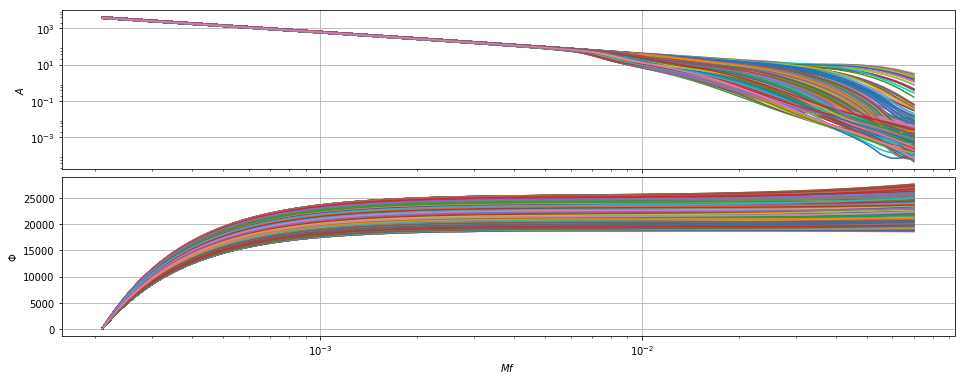
\includegraphics[width=0.49\textwidth]{h_trainingset.png}\\
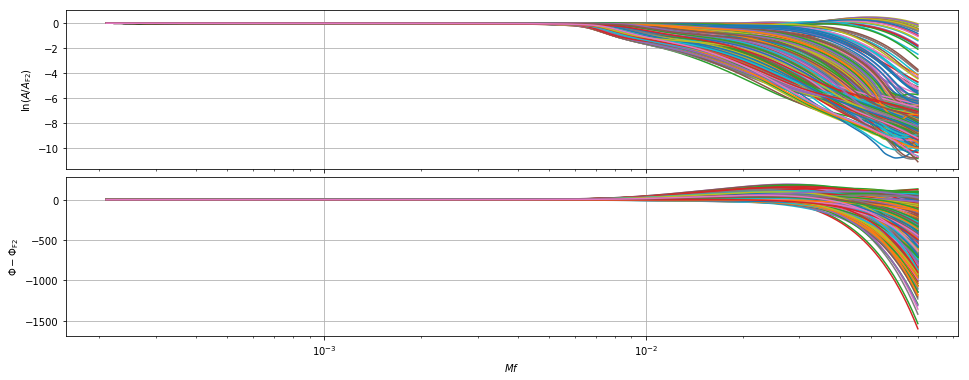
\includegraphics[width=0.49\textwidth]{dh_trainingset.png}
\caption{Training set}
\label{fig:h}
\end{figure}

Although the amplitude and phase are relatively smooth functions, they still span a wide range of values. The phase, for example, spans about $10^4$~rad. Unfortunately, to avoid systematic errors in the tidal parameters, we need phase errors of $\lesssim 1$~rad over most of this frequency range, leading to a requirement on the fractional interpolation error of $\lesssim 10^{-4}$~rad. This is a difficult requirement to achieve in the 5-dimensional parameter space here. However, for aligned-spin waveforms these functions are approximately known analytically from the stationary phase approximation to the post-Newtonian (PN) waveform known as TaylorF2 $\tilde h_{\rm F2}(f; \bx) = A_{\rm F2}(f; \bx) e^{i\Phi_{\rm F2} (f; \bx)}$ [[cite]]. We can therefore evaluate the EOB waveform in terms of the residuals, $\Delta\ln(A)$ and $\Delta\Phi$, between EOB and TaylorF2
\begin{align}
\tilde h(f; \bx) = A_{\rm F2}(f; \bx) e^{i\Phi_{\rm F2}(f; \bx)} e^{\Delta\ln(A)(f; \bx) + i  \Delta\Phi(f; \bx)},
\label{eq:hdecomp}
\end{align}
where
\begin{align}
\Delta\ln(A)(f; \bx) &= \ln\left(\frac{ A(f; \bx) }{ A_{\rm F2}(f; \bx)}\right),\\
\Delta\Phi(f; \bx) & = \Phi(f; \bx) - \Phi_{\rm F2}(f; \bx).
\end{align}
These residuals are shown in Fig.~\ref{fig:h}. For the amplitude, we use the log-ratio instead of the ratio because it guarantees that the amplitude of the reconstructed waveform in Eq.~\eqref{eq:hdecomp} is positive even if interpolation error leads to a negative $\Delta\ln(A)(f; \bx)$. In addition, because the waveform amplitude spans several orders of magnitude after the merger frequency of each waveform, the log-ratio captures this behavior. 

To demonstrate the usefulness of this approach, in Fig.~\ref{fig:phaserange}, we show the range of values of the phase $\Phi$ over the training set $\Phi_{\rm range} = \Phi_{\rm max} - \Phi_{\rm min}$ as well as the range of values of the phase residual $\Delta\Phi$ over the training set $\Delta\Phi_{\rm range} = \Delta\Phi_{\rm max}-\Delta\Phi_{\rm min}$. The range in $\Phi$ can be larger than 1000~radians. The range of $\Delta\Phi$ is 1--2 orders of magnitude smaller, and as a result, the interpolation accuracy requirements are 1--2 orders of magnitude smaller as well. 

\begin{figure}[htb]
\centering
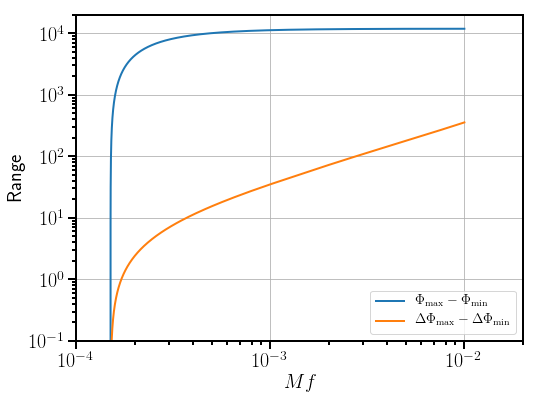
\includegraphics[width=0.49\textwidth]{phaserange.png}
\caption{Range of phase values for training set waveforms. The range is a factor of $\gtrsim 100$ larger for $\Phi$ than for $\Delta\Phi$, 
meaning that the interpolation accuracy requirements are at least $\sim 2$ orders of magnitude less for $\Delta\Phi$.}
\label{fig:phaserange}
\end{figure}

The explicit expressions for the amplitude and phase of the TaylorF2 waveform are as follows. For the amplitude we use the 1PN correction to the leading order waveform.
\begin{equation}
A_{\rm F2} = \sqrt{\frac{5\pi\eta}{24}} x^{-7/4} \left[ 1 + \left(-\frac{323}{224} + \frac{451\eta}{168} \right)x \right],
\end{equation}
where $x=(\pi M f)^{2/3}$ is the standard PN parameter. This differs slightly from the decomposition used by \texttt{lalsuite}. The phase has the schematic form
\begin{align}
\Phi_{\rm F2} =& -2\pi f t_c + \phi_c + \frac{\pi}{4} - \frac{3}{128\eta}x^{-5/2} \left[1 + \right. \\
                        & \left. {\rm PP}(\eta) + {\rm Spin}(\eta, S_1, S_2) + {\rm Tidal}(\eta, \Lambda_1, \Lambda_2)  \right].
\end{align}
We use the point particle terms ${\rm PP}(\eta)$ to 3.5PN order in Eq.~[[]] of Ref.~[[]], the aligned spin terms ${\rm Spin}(\eta, S_1, S_2)$ to 3PN order in Eqs.~[[]] of Ref.~[[]] and Eqs.~[[]] of Ref.~[[]], and the tidal terms ${\rm Tidal}(\eta, \Lambda_1, \Lambda_2)$ to 6PN order in Eqs.~[[]] of Ref.~[[]]. These terms for the phase are exactly as used in the \texttt{lalsuite} waveform \texttt{TaylorF2} [[cite]].




\subsection{Preconditioning the training set waveforms}


We evaluate the EOB waveform with a starting frequency equivalent to 20Hz for a total mass of $M=2M_\odot$ ($Mfwi=0.000197$). In order to take a discrete Fourier transform, we window the start of the waveform with a Planck window [[cite]] in the interval $(Mfwi, Mfwf) = (0.000197, 0.00021)$ to avoid Gibbs oscillations. We then resample the waveform with a spacing $\Delta t/M = 5$, and pad the end of the waveform with zeros such that all waveforms in the training set have the exact same time samples.

After evaluating the discrete Fourier transform, evaluate the residuals $\Delta\ln(A)$ and $\Delta\Phi$ between the EOB and TaylorF2 waveforms. Because waveforms have free time and phase parameters, subtract a linear fit to $\Delta\Phi$ at the beginning of the waveform in the window $(Mf_{fit,i}, Mf_{fit,f}) = 0.00021(1, 1.05)$. The resulting $\Delta\Phi$ is zero and has zero slope at $Mf_{fit,i}$, guaranteeing that the surrogate smoothly matches to TaylorF2 at lower frequencies.

As a result of Gibbs oscillations in the Fourier transformed waveform that weren't completely removed by the Planck waveform as well as from the end of the waveform where the amplitude rapidly drops to zero amplitude after the peak amplitude over $\sim 1$ cycle, small amplitude, high frequency oscillations remain in the residuals $\Delta\ln(A)$ and $\Delta\Phi$. We remove these oscillations using a moving average filter centered on $Mf$ with width $[Mf(1-\Delta Mf), Mf(1+\Delta Mf)]$. We use a width of $\Delta Mf=0.1$ for the amplitude and $\Delta Mf=0.05$ for the phase. 

Finally, we truncate the data to the interval $(Mf_{trunc,i}, Mf_{trunc,f}) = (0.00021, 0.07)$. We note that the gravitational wave frequency at the Schwarzschild ISCO is $Mf_{\rm ISCO} = 1/(6^{3/2}\pi) \approx 0.022$. Although second generation detectors are only marginally sensitive to signals above this frequency, we use the high-frequency cutoff of $Mf_{trunc,f}=0.07$ because some of the EOB waveforms still have enough amplitude at these high frequencies to affect the structure of the surrogate waveform if inverse Fourier transformed back into the time domain.

\red{[[Show plot (?) to validate that waveform is properly conditioned by plotting amplitude/phase as function of waveform parameters at specific frequencies and show that they're smooth functions?]]}


\subsection{Spline interpolation for frequency $f$}

We now seek to interpolate the conditioned and filtered residuals $\Delta\ln(A)(f; \bx)$ and $\Delta\Phi(f; \bx)$. We begin by interpolating as a function of $f$ for fixed $\bx$. The majority of previous papers on gravitational waveform surrogates have used an orthonormal basis of global functions $\hat e_i(f)$ for frequency (or time) interpolation [[cite]]. This type of surrogate is referred to as a reduced order model. For a generic function $g(f; \bx)$, this can be written as $g(f; \bx) \approx \sum_{i=1}^N c_i(\bx) \hat e_i(f)$. The coefficients $c_i(\bx)$ are then interpolated as functions of $\bx$ [[Puerrer]]. Alternatively, using the empirical interpolation method [[cite]], one can re-express these basis functions $\hat e_i(f)$ in terms of empirical interpolating functions $B_j(f)$ and the value of $g(f; \bx)$ at empirical nodes $F_j$ as $g(f; \bx) \approx \sum_{j=1}^N B_j(f) g(F_j; \bx)$. The location of these nodes $F_j$ can be optimized to minimize interpolation errors. This method has been used in Refs.~[[cite]].

For the problem here, we have found that global basis functions do not work well. The residuals are small and smooth at low frequencies and large and noisy at high frequencies. Errors in evaluating $g(F_j;\bx)$ for high frequency can propagate to large errors at low frequencies. Instead, we find that spline interpolation works significantly better. We use 20 frequency nodes $F_j$ log-spaced the interval $[f_{trunc,i}, f_{trunc,f}]$, and evaluate the residuals $\Delta\ln(A)(F_j; \bx)$ and $\Delta\Phi(F_j; \bx)$ at these nodes using GPR discussed below. We then choose third-order spline interpolation to interpolate between these points. The local, third-order polynomials, that are only connected by the requirement of smoothness [[check this]] do not propagate high-frequency errors down to low-frequency errors as significantly.


\subsection{Gaussian process regression for parameters $\bx$}

We use Gaussian process regression to fit the residuals $\Delta\ln(A)(F_j; \bx)$ and $\Delta\Phi(F_j; \bx)$ at the empirical nodes $F_j$ as a function of the waveform parameters. In GPR a function $f(\vec x)$ is described in terms of a mean $m(\vec x)$ and 
covariance $k(\vec x, \vec x')$ between points [[cite RassmussenWilliamsChapter2, IntroArxivPaper]].
\begin{equation}
f(\vec x) \approx \mathcal{GP}(m(\vec x), k(\vec x, \vec x')).
\end{equation}
The mean $m(x)$ can be some parameterized function which is the standard version of regression, 
while $k(\vec x, \vec x')$ is a kernel with tunable hyperparameters that describes the covariance between
the point $\vec x$ and the sampled point $\vec x'$. This covariance can be used to describe features of the function 
not captured by the parameterized mean as well as genuine noise in the data ${\bm y}$. 
For the problem here, we have already subtracted the 
TaylorF2 waveform from EOB waveform, so we set $m=0$ and model the remainder terms purely in terms 
of the covariance $k$. 

In a zero-mean Gaussian process, the data and function $({\bm y}, f_*)$ at the training set and new points $({\bm x}, x_*)$ are
drawn from a multivariate normal distribution
\begin{equation}
\label{eq:gaussian}
\begin{bmatrix}
{\bm y} \\
f_* \\
\end{bmatrix}
\sim \mathcal{N}
\left({\bm 0}, 
\begin{bmatrix}
K & K_*^T \\
K_* & K_{**} \\
\end{bmatrix}
\right)
\end{equation}
where $K = K({\bm x}^i, {\bm x}^j)$ is a matrix, $K_* = K({\bm x}^i, {\bm x}_*)$ is a vector, and $K_{**} = K({\bm x}_*, {\bm x}_*)$ is a scalar.

The conditional probability for $f_*$ given the training set examples ${\bm y}$ with hyperparameters $\theta$ is also a Gaussian
\begin{equation}
f_* | {\bm x}, x_*, {\bm y}, {\bm \theta} \sim \mathcal{N}(\bar f_*, {\rm var}(f_*))
\end{equation}
where the mean and variance are
\begin{align}
\label{eq:mean}
\bar f_* &= K_*^T K^{-1} y \\
\label{eq:var}
{\rm var}(f_*) &= K_{**} - K_*^T K^{-1} K_*.
\end{align}
Eq.~\eqref{eq:mean} is the estimate of the function, and Eq.~\eqref{eq:var} is the estimate of the uncertainty, where we note that the variance does not depend on the data $\bm{y}$.

We use a radial kernel which expresses the covariance in terms of a distance $r$ between points
\begin{equation}
r^2 = (x-x')^T M (x-x'),
\end{equation}
where we choose the matrix M to be diagonal
\begin{equation}
M = {\rm diag}(\ell_1^{-2}, \ell_2^{-2}, \dots, \ell_d^{-2}).
\end{equation}
The tunable hyperparameters $\ell_i$ represent the length scale over which the function $f(x)$ varies in 
each coordinate $x_i$. Specifically, we use the Mat\'{e}rn class of kernels
\begin{equation}
k_{\rm Matern}(r) = \frac{2^{1-\nu}}{\Gamma(\nu)} \left(\sqrt{2\nu} r\right)^\nu K_\nu \left(\sqrt{2\nu} r \right).
\end{equation}
where $K_\nu(x)$ is a modified Bessel function. The value of $\nu$ parameterizes the smoothness of the 
Gaussian Process $f(x)$, and is $k$ times mean-square differentiable if $\nu>k$ [[cite]]. For half-integer values of $\nu$, this 
kernel has a computationally cheap form without special functions, and we have had good results with $\nu=5/2$, 
resulting in a twice-differentiable function. The $\nu=5/2$ kernel is
\begin{equation}
k_{\rm Matern}^{\nu=5/2}(r) = \left(1+\sqrt{5}r + \frac{5r^2}{3}\right) \exp\left(-\sqrt{5}r\right).
\end{equation}

Our final kernel takes the form
\begin{equation}
k(x_p, x_q) = \sigma_f^2 k_{\rm Matern}^{\nu=5/2}(r) + \sigma_n^2 \delta_{pq}
\end{equation}
where $\sigma_f$ is a scale factor that describes the range of values that $f(x)$ takes over the domain, 
and $\sigma_n$ is a noise parameter. The white noise kernel $\sigma_n^2 \delta_{pq}$ (also called a nugget), which is
$\sigma_n^2$ when $x_p=x_q$ and zero otherwise, is generically used for numerical stability, but also parameterizes
noise in the data ${\bm y}$. In our case, the training set waveforms which are evaluated, tapered, and 
Fourier transformed numerically have numerical noise that we will estimate by optimizing the hyperparameters.
The hyperparameters now are $\theta = \{\sigma_f, \ell_q, \ell_{S_1}, \ell_{S_2}, \ell_{\Lambda_1}, \ell_{\Lambda_2}, \sigma_n\}$.

[[In principle, one can select the optimal class of kernels using k-fold or leave-one-out cross validation. We have also tried the 
more common infinitely differentiable squared exponential kernel. However, we found it difficult to reliably tune the 
hyperparameters for the problem here.]]

In order to estimate the hyperparameters, we use the above assumption (Eq.~\eqref{eq:gaussian}) that the joint distribution of 
the data ${\bm y}$ is a multivariate Gaussian which has the following distribution
\begin{equation}
\ln p({\bm y} | {\bm x}, {\bm \theta}) = -\frac{1}{2}{\bm y}^T K^{-1} {\bm y} - \frac{1}{2} \ln |K| - \frac{d}{2} \ln 2\pi.
\end{equation}
This is the log-likelihood for ${\bm y}$ given the hyperparameters ${\bm \theta}$, and we can find the posterior for ${\bm \theta}$
given ${\bm y}$ using Bayes' theorem
\begin{equation}
p({\bm \theta} | {\bm x}, {\bm y}) \propto p({\bm \theta}) p({\bm y} | {\bm x}, {\bm \theta}).
\end{equation}
The prior $p({\bm \theta})$ is typically uniform and used to set the bounds on ${\bm \theta}$. If interested in the distribution of the 
hyperparamaters, one can sample this posterior with, for example, Markov chain Monte Carlo. However, for the problem here, we are
simply interested in finding the maximum of the posterior. To do this, we use the \texttt{gaussian\_process} module in the
\texttt{scikit-learn} package [[cite]]. Finally, with the optimized hyperparameters ${\bm \theta}$, Eq.~\eqref{eq:var} is the 
interpolating function. We note that evaluating Eq.~\eqref{eq:var}, is an $\mathcal{O}(N)$ operation if the vector $K^{-1}{\bm y}$ is
precomputed.


\subsection{Iterative construction of training set}


In the subsections below we will build our surrogate with the aim of using as few waveform evaluations as possible. We do this because EOB models of BNS systems are already expensive, and we would like a method that extends to higher dimensions and more expensive simulations such as numerical relativity simulations. A general overview of the process we have used is as follows:
\begin{enumerate}
\item Select an initial, sparse set of waveform parameters $\bx$ that cover the parameter space using a Latin Hypercube Design (LHD).

\item Evaluate the initial training set of EOB waveforms $h(t;\bx)$ and condition them to produce smoothed, frequency-domain waveforms $\tilde h(f;\bx)$.

%\item Construct separate orthonormal, reduced bases for the amplitude $A(f;\bx)$ and phase $\Phi(f;\bx)$ of the training set waveforms. Then, use the empirical interpolation method (EIM) to generate separate sets of frequency-dependent empirical interpolating functions for the amplitude $B^A_j(f)$ and phase $B^\Phi_j(f)$.

\item Choose interpolation nodes.

%\item For each empirical interpolating function, interpolate the amplitude $A(F^A_j;\bx)$ or phase $\Phi(F^\Phi_j;\bx)$ at the associated frequency nodes $F^A_j$ or $F^\Phi_j$, respectively, as a function of the waveform parameters $\bx$ using GPR.

\item GPR


\item With the resulting surrogate model and GPR uncertainty estimates, iteratively choose the points in parameter space with the largest estimated waveform errors. Then, generate these waveforms and add them to the initial training set.

\item Reconstruct the surrogate model with the updated training set. This can be repeated as necessary with additional training set waveforms.

\end{enumerate}

In constructing a surrogate model, we will need to interpolate several quantities as a function of the five
waveform parameters ${\bm x}$.
Most multivariate interpolation techniques (e.g. tensor spline or Chebyshev interpolation) 
require a function to be sampled on a rectangular grid, and thus suffer from the curse of dimensionality; 
the number of samples grows exponentially with the dimension $d$ ($N^d$ for $N$ samples per dimension).
In the 5-dimensional problem discussed here, $10^5$ waveform evaluations are needed for only 10 samples per parameter.
At 10 minutes--1 hour per EOB waveform on a standard CPU, this is at the limit of what is reasonable.

However, there are other methods such as Gaussian Process Regression (GPR), discussed below, that allow nonuniform designs.
One such standard design is a Latin Hypercube Design (LHD). An LHD with $N$ samples divides each dimension uniformly into $N$
grid points per dimension for a total of $N^d$ possible locations. However, for each dimension each of the $N$ values is sampled 
exactly once. This has the convenient property that the samples are non-collapsing; if one of the parameters is much less 
significant than other parameters, samples are not wasted on that parameter, as they would be with a uniform grid. And, a projection
onto a subspace is still a LHD. [[Also, each dimension is uniformly sampled which is not the case for MC sampling.]]

As an example of the usefulness of noncollapsing designs, the tidal parameters have a minimal impact on the waveform
at low frequencies, so it wouldn't make sense to densely sample a grid of tidal parameters at low frequencies. However, near
the merger the tidal parameters can be a important as the spin parameters. One therefore might want more samples for the tidal
parameters and less samples for the spin. However, due to the expense of the wavefroms we must use the same grid of waveforms 
for low and high frequencies. A LHD, with its noncollapsing property, bypasses this problem. 

For an LHD there are $(N!)^d$ possible designs, and a standard requirement is that the LHD be space-filling, meaning that the 
points are as far apart as possible from each other. (See [[cite]] for a review of methods for optimizing the placement of samples.) 
The measure used here is that we maximize the minimum Euclidean distance between any two samples [[cite]]. We do this by 
sampling $xxx$ random designs and choosing the one with the maximum minimum distance.

For a smooth approximately monotonic function in $d$-dimensions, standard lore is that $10d$ samples are needed to interpolate 
a function with GPR [[cite]] [[To what accuracy]]. We therefore construct our initial training set with 50 waveform samples, and use 
these waveforms to construct the reduced basis and perform interpolation with GPR. Once an initial surrogate model is constructed,
we will use the GPR error estimate to choose new waveforms to add to the training set, and update the surrogate model.

\begin{figure}[htb]
\centering
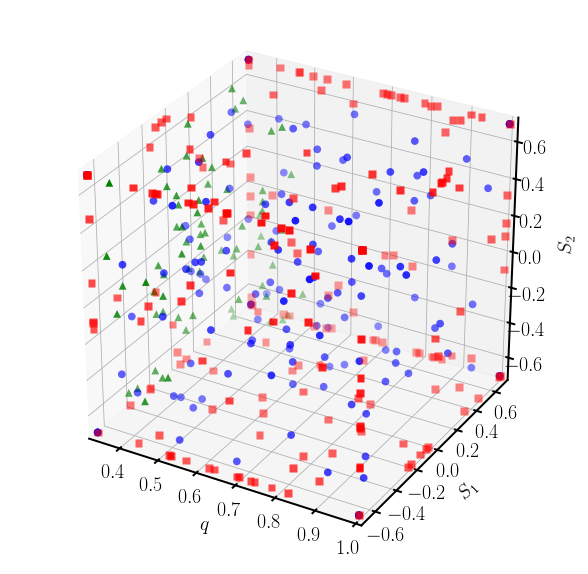
\includegraphics[width=0.49\textwidth]{trainingset3d.png}\\
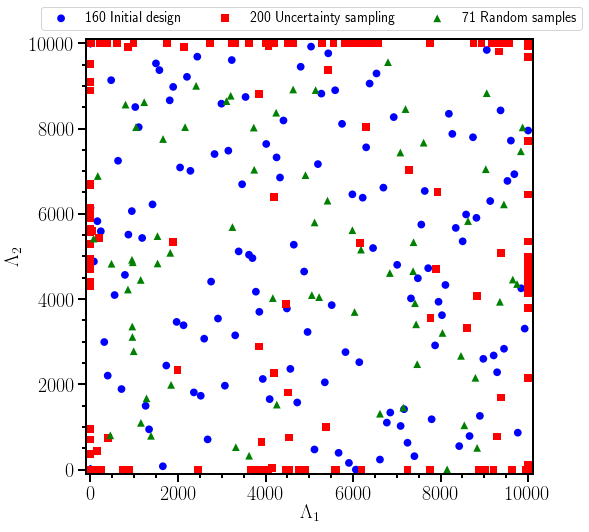
\includegraphics[width=0.49\textwidth]{trainingset2d.png}
\caption{Projection of the sampled waveforms onto the three-dimensional subspace $\{q, S_1, S_2\}$ (top)
and the two-dimensional subspace $\{\Lambda_1, \Lambda_2\}$ (bottom). The 160 black circles were used for the initial
training set (32 corner points + 128 LHD points) that generated the initial surrogate. The 200 red squares were generated
using uncertainty sampling from the GPR error estimate of the RMS phase error at the empirical nodes. 
}
\label{fig:LHD}
\end{figure}


Once we have an initial surrogate model, we can choose new training set samples by iteratively searching the parameter space
for new points ${\bm x}$ that maximize some error criterion. The quantity that we use is the distinguishability between the
EOB waveform and its surrogate [[cite]]
\begin{equation}
|\delta h | = \sqrt{(h - h_{\rm Sur} | h - h_{\rm Sur})}.
\end{equation}
For an initial training set with N samples, this function has $\sim N$ local maxima. We use Monte Carlo sampling with ~100,000
samples and choose the point with the largest distinguishability [[for now. Could also use multistart optimization.]] to find the 
approximate global maximum. Because $|\delta h |$ is an expensive function that requires an EOB or NR evaluation, 
we approximate it as follows:

[[Your inexpensive way of approximating $|\delta h |$ that does not depend on $h_{\rm EOB}$ here.]]
\begin{equation}
\label{eq:distinguish}
|\delta h | \approx blah.
\end{equation}


With this new sample, one could evaluate the waveform at the new point and reconstruct the surrogate model, then iterate.

Reconstructing the surrogate for each new sample is inexpensive compared to the time needed to simulate a new NR waveform. 
However, even for NR waveforms, one often wants to perform $N_{\rm new}$ new waveform simulations in parallel. 
We therefore need a method for optimally choosing $N_{\rm new}$ new samples. One could simply choose the 
$N_{\rm new}$ local maxima with the largest $|\delta h |$. However, there is a more optimal way of iteratively finding new points.
If we hold the hyperparameters ${\bm \theta}$ fixed, we note that the GPR error estimate (Eq.~\eqref{eq:var}) does not depend
on the data ${\bm y}$, just on the samples ${\bm x}$. Therefore, the approximate $|\delta h |$ (Eq.~\eqref{eq:distinguish}) does not depend
on the new samples either. The method uses the idea of uncertainty sampling [[cite]] but without updating the hyperparameters
after each new point is chosen. The algorithm for choosing the new points is as follows.

While $|\delta h |_{\rm max} > \epsilon$:
\begin{enumerate}
\item Construct the GPR error functions (Eq.~\eqref{eq:var}) at each of the empirical nodes $F^A_j$ and $F^\Phi_j$.
In practice this can be done by specifying the samples ${\bm x}$, the hyperparameters ${\bm \theta}$, and dummy 
data ${\bm y}={\bm 1}$. These GPR error functions are the input to Eq.~\eqref{eq:distinguish}.

\item Find $({\bm x}_{\rm max}, |\delta h |_{\rm max})$ that maximizes Eq.~\eqref{eq:distinguish} over the parameter space. 
\item Add ${\bm x}_{\rm max}$ to the list of samples: ${\bm x} = [{\bm x}, {\bm x}_{\rm max}]$.
\end{enumerate}
These new waveforms can now be evaluated in parallel.

[[The methods used here fall under the terms active learning and Bayesian optimization [[cite]]. The specific method being used is
uncertainty sampling [[cite]]. The parallelization method I am using I have not seen in the literature. Is it actually new? Ask Niki.]]


[[Another method you could try is k-means clustering of the mismatch for your validation set (using mismatch above some threshold), 
where you have $k=N$, because there will
be $\sim N$ local maxima of the mismatch. Within each cluster, choose the waveform with the largest mismatch and add it to the
training set. This way you only use one new point per local maximum region. You could do the same thing with the Fisher matrix
systematic error calculation instead of the mismatch if that's a better quantity to use.]]

\begin{figure}[htb]
\centering
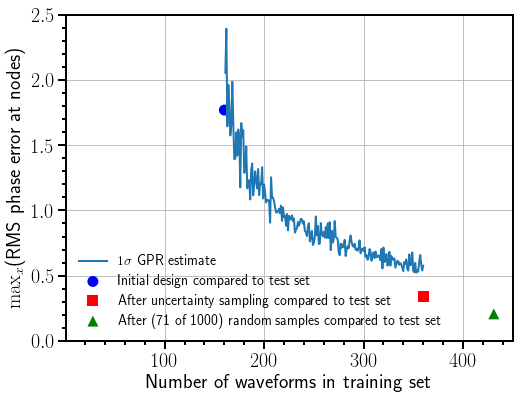
\includegraphics[width=0.49\textwidth]{uncertaintysampling.png}
\caption{Estimated RMS phase error as function of number of sampled points}
\label{fig:uncsamp}
\end{figure}


\subsection{Surrogate waveform evaluation}

Given the interpolating functions for the amplitude and phase residuals $\{\mathcal{I}_{\rm GPR}[\Delta\ln A_j](\bx)\}$ and $\{\mathcal{I}_{\rm GPR, j}[\Delta\Phi_j](\bx)\}$ evaluated at the frequency nodes $\{F_j\}$, we can now reconstruct the frequency-domain waveform. The surrogates for the residuals $\Delta\ln A_S(Mf;\bx)$ and $\Delta\Phi_S(Mf;\bx)$ are constructed by interpolating between the nodes $\{F_j\}$ with cubic splines:
\begin{align}
\Delta\ln A_S(Mf;\bx) &= \mathcal{I}_{\rm Spline}[\{\mathcal{I}_{\rm GPR}[\Delta\ln A_j](\bx)\}](Mf),\\
\Delta\Phi_S(Mf;\bx) &= \mathcal{I}_{\rm Spline}[\mathcal{I}_{\rm GPR}[\{\Delta\Phi_j](\bx)\}](Mf).
\end{align}
We set these functions to 0 below the first frequency node $MF_0 =  Mf_{trunc,i}$ so that the waveform transitions to TaylorF2 at lower frequencies. With the analytic expressions for $A_{\rm F2}(Mf;\bx)$ and $\Phi_{\rm F2}(Mf;\bx)$ and the interpolated expressions $\Delta\ln A_S(Mf;\bx)$ and $\Delta\Phi_S(Mf;\bx)$, the final surrogates for the amplitude and phase are
\begin{align}
A_S(Mf;\bx) &= A_{\rm F2}(Mf;\bx) \exp\left[ \Delta\ln A_S(Mf;\bx) \right] \\
\Phi_S(Mf;\bx) &= \Phi_{\rm F2}(Mf;\bx) + \Delta\Phi_S(Mf;\bx).
\end{align}
In physical units the $+$ and $\times$ polarizations of the waveform are then 
\begin{align}
\tilde h_+(f; \bx) &= \frac{1}{2}(1+\cos^2\iota) \frac{G^2 M^2}{c^5 d} A_S\left(\frac{GMf}{c^3}; \bx\right) \nonumber \\
& \times \exp\left[i \Phi_S\left(\frac{GMf}{c^3}; \bx\right)\right] \\
\tilde h_\times(f; \bx) &= \cos\iota \frac{G^2 M^2}{c^5 d} A_S\left(\frac{GMf}{c^3}; \bx\right) \nonumber \\
& \times \exp\left[i \Phi_S\left(\frac{GMf}{c^3}; \bx\right) + i \frac{\pi}{2}\right]
\end{align}
where $\iota$ is the inclination angle.



%% ________________________________________________________
\section{Results}

\subsection{Accuracy}

The accuracy of the surrogate can be assessed by comparing it to a test set of waveforms with randomly sampled parameters. We evaluate an additional 1000 waveforms randomly sampled in parameter space using the same distribution discussed above to generate the last 1000 waveforms for the training set.

A common measure of the surrogate model accuracy is the mismatch between 
the surrogate model and the original EOB waveform.
The mismatch represents the loss in signal-to-noise ratio that would result 
from using the surrogate model instead of the original EOB waveform. 
It is defined by the deviation from a perfect overlap after aligning the two waveforms
using the time and phase free parameters $t_0$ and $\phi_0$:
\begin{equation}
\mathcal{M} = 1 - \max_{t_0, \phi_0} \frac{(h_{\rm EOB}, h_{\rm Sur})} {\sqrt{(h_{\rm EOB}, h_{\rm EOB}) (h_{\rm Sur}, h_{\rm Sur})}}.
\end{equation}
The inner product here  is the integral of the Fourier transformed waveforms $\tilde h(f)$ weighted by the noise power spectral 
density (PSD) $S_n(f)$ of the detector:
\begin{equation}
(h_1, h_2) = 4 \Re \int_{f_{\rm low}}^{f_{\rm high}} \frac{\tilde h_1(f) \tilde h^*_2(f)} {S_n(f)} df.
\end{equation}

In Fig.~\ref{fig:mismatch}, we show the distribution of mismatch $\mathcal{M}$ between our surrogate
and the $10^3$ randomly sampled EOB waveforms. We use the design sensitivity aLIGO PSD~\cite{Aasi:2013wya} and
a sampling rate of 4096~Hz. Our integration bounds are $f_{\rm low} = x$~Hz and the Nyquist frequency
$f_{\rm high} = 2048$~Hz. Because the surrogate can be rescaled with mass,
we show results for the smaller mass $M_B$ fixed at $1M_\odot$ or fixed at $2M_\odot$.
[[This is all wrong. Fix it.]]
We compare this mismatch to that of th

\begin{figure}[htb]
\centering
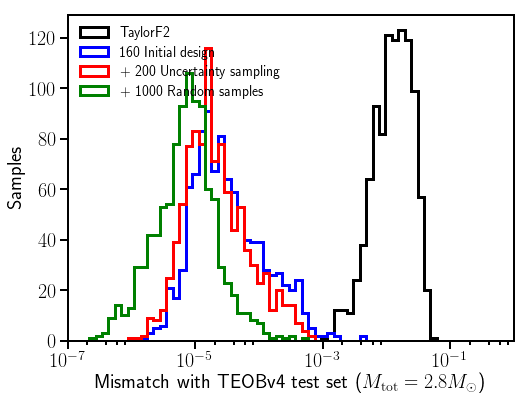
\includegraphics[width=0.49\textwidth]{mismatch.png}
\caption{Mismatch}
\label{fig:mismatch}
\end{figure}

\begin{figure}[htb]
\centering
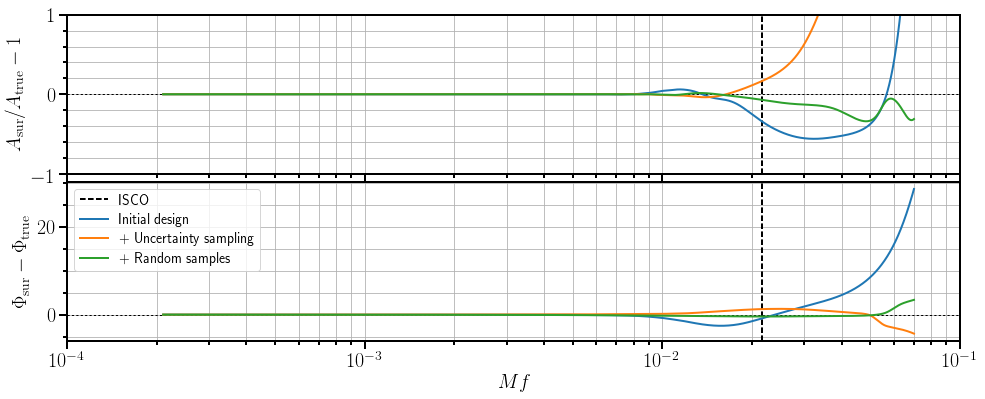
\includegraphics[width=0.49\textwidth]{htildemaxerror.png}
\caption{Amplitude and phase errors as functions of frequency for the waveform parameters $\bx$ that gave the largest mismatch with the test-set waveforms.}
\label{fig:maxmismatch}
\end{figure}

To demonstrate that we can correctly recover the behavior of the original unfiltered time-domain EOB waveform, we inverse Fourier transform the surrogate and compare it to the EOB waveform. In Fig.~\ref{fig:maxmismatchtd} we compare the surrogate to the test set waveform that had the largest mismatch. We align the two waveforms in time and phase by maximizing the overlap at early times in the interval $-200,000 < t/M < -100,000$. The two waveforms are nearly identical except during the last $\sim 2$ cycles where the surrogate peaks in amplitude before the EOB waveform.

\begin{figure}[htb]
\centering
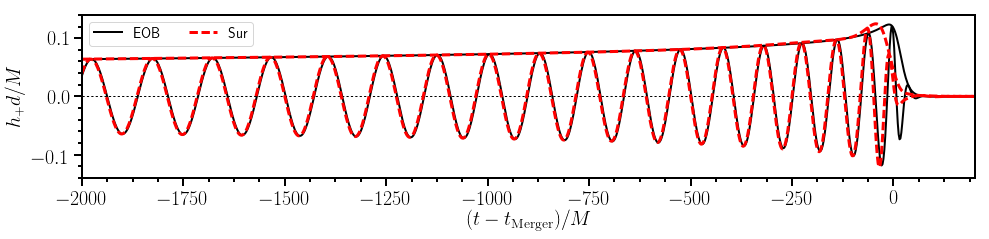
\includegraphics[width=0.49\textwidth]{hmaxerror.png}
\caption{Inverse Fourier transformed surrogate compared to the original EOB waveform.}
\label{fig:maxmismatchtd}
\end{figure}




%\begin{figure}[htb]
%\centering
%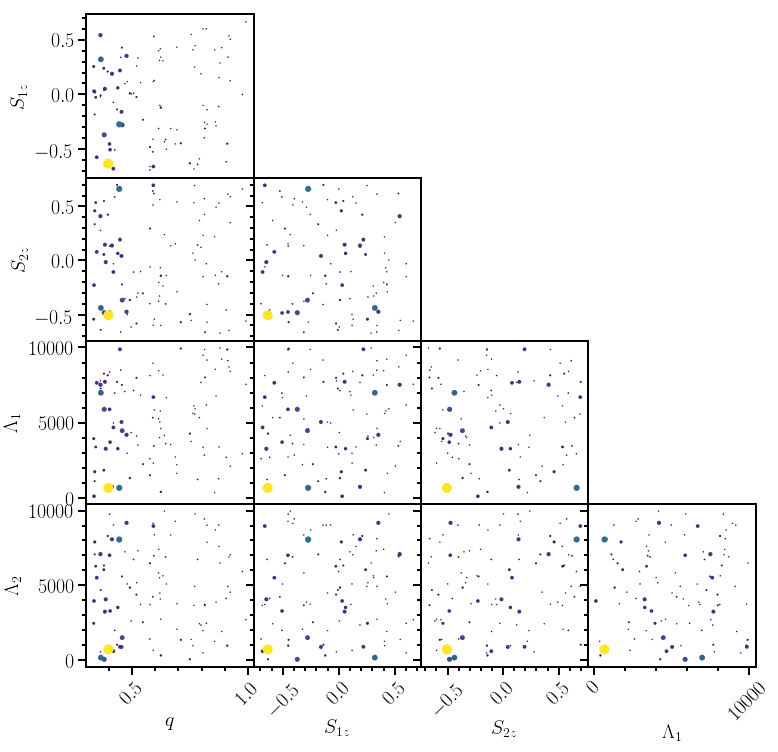
\includegraphics[width=0.49\textwidth]{mismatchtrianglem10.png}
%\caption{Mismatch for systems with $m_2=1M_\odot$.}
%\label{fig:mismatchtriangle}
%\end{figure}









%--Fisher matrix systematic error. (See spin NSBH paper.)
%
%--Phase error. (needs to be significantly smaller than tidal effects) Use this for order of magnitude estimate of required
%accuracy.
%
%\begin{figure}[htb]
%\centering
%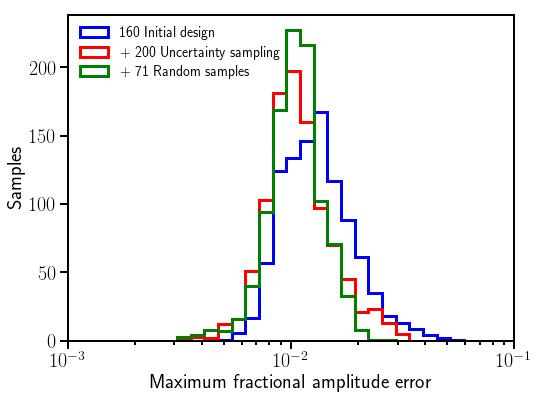
\includegraphics[width=0.49\textwidth]{maxamphist.png}
%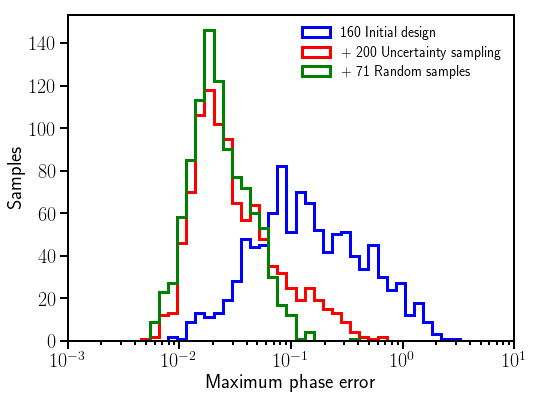
\includegraphics[width=0.49\textwidth]{maxphasehist.png}
%\caption{Amplitude and phase error.}
%\label{fig:ampphaseerr}
%\end{figure}
%


%--distinguishability
%
%--Fisher matrix systematic error.



\subsection{Timing}

Although optimizing the hyperparameters scales with number of samples $n$ as $\mathcal{O}(n^3)$
due to the required matrix inversion, the evaluation time of a stored GPR scales as $\mathcal{O}(n)$.
The evaluation time for the waveform functions will therefore be $\mathcal{O}(n(N_A+N_\Phi))$.

The surrogate has a fixed time of $\sim 50$~ms to evaluate the GPR at each node then evaluate the amplitude
and phase at the log-spaced frequencies. Then, there is an additional cost to resample the amplitude and phase
at uniformly-spaced frequencies with interpolation, and finally evaluating $\tilde h_+$ and $\tilde h_\times$. 
Below 50~Hz the surrogate is faster than all models except TaylorF2 [[you didn't try PhenomP etc.]], and below
18~Hz it is faster than TaylorF2. 

\begin{figure}[htb]
\centering
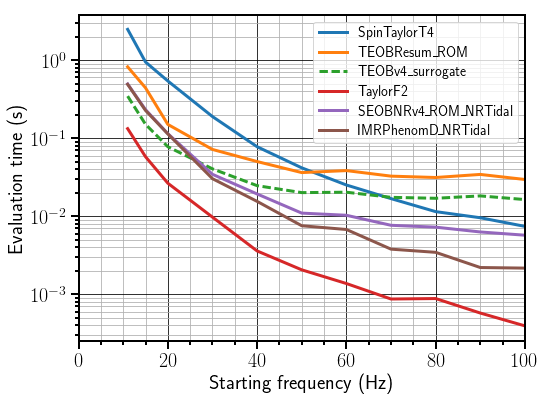
\includegraphics[width=0.49\textwidth]{timing.png}
\caption{Waveform evaluation time as a function of the waveform starting frequency. The time-domain waveforms
were sampled at 4096~Hz then Fourier transformed. The frequency-domain waveforms used the
same frequency samples as the Fourier transformed time-domain waveforms.}
\label{fig:timing}
\end{figure}

--Frequency domain allows for evaluating likelihood with non-uniform sampling.

--Can construct a ROQ of the model if needed.

%\subsection{Parameter estimation}
%
%--Can only include this section if there's a LAL version. Should you bother?


\section{Discussion and future work}

We have constructed a fast frequency-domain surrogate of the most accurate BNS waveform currently available for data analysis. This aligned-spin model, TEOBv4, incorporates the tidally induced $\ell=2$ and 3 multipole moments as well as the effect of dynamical tides as the excitation approaches the $\ell=2$ and 3 f-mode frequencies. We have achieved mismatches of no more than $7 \times 10^{-4}$ and phase errors of $\lesssim 1$~rad up to the merger frequency. These are sufficient to not bias results in any of the parameters.

The evaluation time has a flat cost of $\sim 0.02$~s to perform the GPR interpolation at each node. The rest of the time is spent resampling the waveform with spline interpolation. For a starting frequency of 10~Hz, this takes 0.3~s when the waveform is matched with data uniformly sampled at 4096Hz. For a starting frequency of 30~Hz, the total evaluation time is 0.04~s. For current parameter estimation codes, this is sufficient. However, one could further improve run times using reduced order quadrature [[cite]] which requires frequency-domain waveforms, or adaptively sampled likelihood evaluation [[cite]].

The hierarchical method presented here, where we begin with the analytic TaylorF2 reference model then make a surrogate of the residual, can be used to further improve the waveform model. For example, one could build a surrogate for numerical BNS simulations using TEOBv4\_surrogate as the base model, and constructing a surrogate of the residual. Such a model would have the accuracy of EOB below $\sim 400$~Hz and the accuracy of numerical simulations for the last several cycles before merger (once numerical simulations can be proven to be more accurate than EOB [[cite Tim? Kyohei?]]). Using GPR and uncertainty sampling discussed above, one could optimally choose the waveform parameters for the numerical simulations, and run them in parallel to build the training set. Because the difference between TEOBv4 and numerical BNS simulations is exceptionally small, one would not need a high fractional accuracy for a surrogate of the difference, and 10--100 waveforms may be sufficient.

This model notably does not include two effects that can be important for systems with large spin. The first is the spin-induced quadrupole moment $Q$ that effects the waveform phase at 2PN order [[cite Poisson]]. The easiest way to correct for this effect is to simply add this 2PN term to the TaylorF2 reference waveform. One can use the universal relation between the quadrupole moment $Q$ and the tidal parameter $\Lambda$ as was done with the other NS matter parameters. Once this effect is incorporated into the EOB model, one could easily rebuild the surrogate presented in this paper to incorporate this effect.

The second effect is precession for non-aligned spins. Although none of the EOB models currently available include both tidal effects and precession, there are ways to boost this waveform model to a precessing frame, and approximately incorporate precession. For example, Chatziioanno et al. have analytically solved the 2PN-accurate precession equations for generic spins. This only works for systems that do not include transitional precession, as is unlikely for low mass ratio BNS systems [[cite]]. Using stationary uniform asymptotics, they can also analytically Fourier-transform the solution. Importantly, one is free to specify the frequency-domain amplitude and phase evolution, such as the TEOBv4\_surrogate here, for the waveform in the co-precessing frame. This approach would provide a fast, accurate model for BNS systems with tides and generic spins.


%% ________________________________________________________
\begin{acknowledgments}

BL thanks the participants of the Bayesian Methods in Nuclear Physics workshop at the Institute for Nuclear Theory where many of the methods used here were discussed. BL, MP, and AT were supported by... 

\end{acknowledgments}


%% ________________________________________________________
%\bibliographystyle{revtex}     
\bibliography{paper,refs}  



\end{document}











%\section{Old Junk text}
%
%
%
%\sout{A time-domain surrogate has the advantage that significantly less processing of the original waveform is needed, resulting in a surrogate that typically more accurately reproduces the original waveform model.}
%%A frequency-domain surrogate, on the other hand, requires windowing of the Fourier transformed waveform to avoid Gibbs oscillations. For the beginning of the waveform, one can simply begin at a lower frequency, window the waveform, then truncate the Fourier-transformed waveform above some desired starting frequency. 
%
%
%\sout{As we will show in Sec.~[[]], these high-frequency Gibbs oscillations in the amplitude of the Fourier transformed waveform are a genuine feature of BNS waveforms unlike BBH waveforms which typically taper over a larger number of GW cycles during their ringdown. These oscillations make it difficult to construct a surrogate. However, we will show that smoothing these oscillations in the Fourier transformed waveform with a moving average filter leads to a surrogate that is sufficiently faithful to the original time-domain model. Another important advantage is that a surrogate of $\tilde h(f;\bx)$ bypasses the need to evaluate the Fourier transform at each waveform evaluation for parameter estimation. And, as we shall see, a frequency-domain surrogate can be trivially attached to analytic models that are accurate at low-frequencies, such as TaylorF2, making analysis for third-generation detectors which are sensitive at lower frequencies easier. Finally, methods for speeding up the likelihood evaluation in parameter estimation such as reduced order quadrature typically require a fast frequency-domain model for calculating the appropriate weights online [[cite]]. For these reasons we will construct a surrogate of $\tilde h(f;\bx)$.}





\begin{widetext}
\begin{align}
\Lambda_{2,\textrm{dyn}}^{\textrm{(A,B)}}(u) = &\frac{\lambda_{2}^{\textrm{(1,2)}}}{M^5} \left\{\frac{1}{4} + \frac{3}{4} \left(\frac{\omega^{(1,2)}_{f,2}}{2\Omega}\right)^2\left[\frac{4\Omega^2}{(\omega^{(1,2)}_{f,2})^2 - 4\Omega^2} + \frac{10}{3Q}\right.\right. \nonumber\\
&\left.\left.+\sqrt{\frac{\pi}{3}}\frac{1}{\epsilon_{1,2}}\left[(1 + 2\mathcal{S}{(y_{1,2})})\cos{\left(\frac{\pi}{2}y^2_{1,2}\right)} - (1 + 2\mathcal{C}{(y_{1,2})})\sin{\left(\frac{\pi}{2}y_{1,2}^2\right)}\right]\right]\right\}\,,\\
\Lambda_{3,\textrm{eff}}^{\textrm{(1,2)}} (u)= &\frac{\lambda_{3}^{\textrm{(1,2)}}}{M^7} \left\{\frac{3}{8} + \frac{(\omega^{(1,2)}_{f,3})^2}{\Omega^2}\left(\frac{25}{48 O_{1,2}} + \frac{5}{72}\frac{9\Omega^2}{(\omega^{(1,2)}_{f,3})^2-9\Omega^2}\right)\right. \nonumber\\
&\left.+ O_{1,2}\left[\cos{(w^2)}\left(\frac{1}{2} +\mathcal{S}(sqrt2pi*w)\right) - \sin{(w^2)}\left(\frac{1}{2} + \mathcal{C}(sqrt2pi*w)\right)\right]\right\}\,,
\end{align}
\end{widetext}
where $\lambda_{2}^{\textrm{(1,2)}}$ are the (constant) adiabatic values of the quadrupolar tidal polarizabilities, $\lambda_{3}^{\textrm{(1,2)}}$ are the (constant) adiabatic values of the octupolar tidal polarizabilities, $\omega^{(1,2)}_{f,2}$ are the quadrupolar $f$-mode frequencies, $\omega^{(1,2)}_{f,3}$ are the octupolar $f$-mode frequencies, $\mathcal{S}$ is the Fresnel sine integral, $\mathcal{C}$ is the Fresnel cosine integral, $\epsilon_{1,2} = 2^{19/3}\nu (M\omega^{(1,2)}_{f,2})^{5/3}/5$,   $y_{1,2}=\sqrt{3/(\pi \epsilon)} Q_{1,2}/5$, and $Q_{1,2} = 4- 2^{1/3}(M\omega^{(1,2)}_{f,2})^{5/3}u^{-5/2}$. 
, $w_{1,2}=O_{1,2}/(4\,3^{2/3}\sqrt{10}(M\omega^{(1,2)}_{f,3})^{5/6}\sqrt{\nu})$, $O_{1,2}=5\sqrt{5\pi}/u^3(M\omega^{(1,2)}_{f,3})^{7/6}/(192\,3^{2/3}\sqrt{\nu})$.

